\documentclass[twocolumn, twocolappendix]{aastex63}

% \documentclass[linenumbers,preprint2,tighten,trackchanges]{aastex631}
%\documentclass[nolinenumbers,preprint2,tighten]{aastex631}
\hypersetup{filecolor=cyan,urlcolor=magenta} %citecolor=green, linkcolor=red,
\newcommand{\vdag}{(v)^\dagger}
\newcommand\aastex{AAS\TeX}
\newcommand\latex{La\TeX}
\usepackage{amsmath}	% Advanced maths commands
\usepackage{amssymb}	% Extra maths symbols
\usepackage{mathrsfs}

\usepackage{bigints}
\usepackage{CJK}

\newcommand{\Msun}{M_\odot}
\newcommand{\Msunyr}{M_\odot~{\rm yr}^{-1}}
\newcommand{\Mh}{M_\mathrm{h}}
\newcommand{\Mbh}{M_\bullet}
\newcommand{\Mseed}{M_\mathrm{seed}}
\newcommand{\zseed}{z_\mathrm{seed}}
\newcommand{\hh}{\mathrm{H_2}}
\newcommand{\CII}{\mathrm{C_{II}}}
\newcommand{\vbsm}{v_\mathrm{bsm}}
\newcommand{\jlw}{J_{\rm LW}}
\newcommand{\Mdot}{\dot{M}}
% \newcommand{\tlife}{t_\mathrm{life}}
\newcommand{\tlife}{\tau}
\newcommand{\fseed}{f_\mathrm{seed}}
\newcommand{\fobsc}{f_\mathrm{obsc}}
\newcommand{\Nt}{N_\mathrm{t}}
\newcommand{\Muv}{M_{1450}}
\newcommand{\Lbol}{L_\mathrm{bol}}
\newcommand{\fbol}{f_\mathrm{bol}}
\newcommand{\D}{\mathrm{d}}

\newcommand{\red}[1]{\textcolor{red}{ #1}}
\newcommand{\blue}[1]{\textcolor{blue}{ #1}}

\defcitealias{2010AJ....140..546W}{W10}
\defcitealias{2018ApJ...869..150M}{M18}


%\received{March 1, 2021}
%\revised{April 1, 2021}
%\accepted{\today}

%% The following command can be used to set the latex table counters.  It
%% is needed in this document because it uses a mix of latex tabular and
%% AASTeX deluxetables.  In general it should not be needed.
\setcounter{table}{1}

%%%%%%%%%%%%%%%%%%%%%%%%%%%%%%%%%%%%%%%%%%%%%%%%%%%%%%%%%%%%%%%%%%%%%%%%%%%%%%%%
%%
%% The following section outlines numerous optional output that
%% can be displayed in the front matter or as running meta-data.

\shorttitle{BH growth toward $z=$ 6 BHMF \& QLF}
 \shortauthors{Li et al.}
%%
%% You can add a light gray and diagonal water-mark to the first page 
%% with this command:
% \watermark{DRAFT}
%% where "text", e.g. DRAFT, is the text to appear.  If the text is 
%% long you can control the water-mark size with:
%% \setwatermarkfontsize{dimension}
%% where dimension is any recognized LaTeX dimension, e.g. pt, in, etc.
%%
%%%%%%%%%%%%%%%%%%%%%%%%%%%%%%%%%%%%%%%%%%%%%%%%%%%%%%%%%%%%%%%%%%%%%%%%%%%%%%%%
\graphicspath{{./}{../figs/}}
% \graphicspath{{./}{figures/}{figs/}}
%% This is the end of the preamble.  Indicate the beginning of the
%% manuscript itself with \begin{document}.

\begin{document}
\begin{CJK*}{UTF8}{gbsn}

\title{Draft}

\correspondingauthor{}
\email{}

\author[0000-0001-9840-4959]{Wenxiu Li}
\affiliation{Department of Astronomy, School of Physics, Peking University, Beijing, 100871, China}
\author[0000-0001-9840-4959]{Kohei Inayoshi}
\affiliation{Kavli Institute for Astronomy and Astrophysics, Peking University, Beijing 100871, China}
\author[0000-0001-9840-4959]{Masafusa Onoue}
\altaffiliation{Kavli Astrophysics Fellow}
\affiliation{Kavli Institute for Astronomy and Astrophysics, Peking University, Beijing 100871, China}
\affiliation{Kavli Institute for the Physics and Mathematics of the Universe (Kavli IPMU, WPI), The University of Tokyo, Chiba 277-8583, Japan}

%% A significant change from earlier AASTEX versions is in the structure for 
%% calling author and affiliations. The change was necessary to implement 
%% auto-indexing of affiliations which prior was a manual process that could 
%% easily be tedious in large author manuscripts.
%%
%% Use \affiliation for affiliation information. The old \affil is now aliased
%% to \affiliation. AASTeX v6.31 will automatically index these in the header.
%% When a duplicate is found its index will be the same as its previous entry.
%%
%% Note that \altaffilmark and \altaffiltext have been removed and thus 
%% can not be used to document secondary affiliations. If they are used latex
%% will issue a specific error message and quit. Please use multiple 
%% \affiliation calls for to document more than one affiliation.
%%
%% The new \altaffiliation can be used to indicate some secondary information
%% such as fellowships. This command produces a non-numeric footnote that is
%% set away from the numeric \affiliation footnotes.  NOTE that if an
%% \altaffiliation command is used it must come BEFORE the \affiliation call,
%% right after the \author command, in order to place the footnotes in
%% the proper location.
%%
%% Use \email to set provide email addresses. Each \email will appear on its
%% own line so you can put multiple email address in one \email call. A new
%% \correspondingauthor command is available in V6.31 to identify the
%% corresponding author of the manuscript. It is the author's responsibility
%% to make sure this name is also in the author list.
%%
%% While authors can be grouped inside the same \author and \affiliation
%% commands it is better to have a single author for each. This allows for
%% one to exploit all the new benefits and should make book-keeping easier.
%%
%% If done correctly the peer review system will be able to
%% automatically put the author and affiliation information from the manuscript
%% and save the corresponding author the trouble of entering it by hand.

%\correspondingauthor{August Muench}
%\email{greg.schwarz@aas.org, gus.muench@aas.org}

% \author[0000-0002-1044-4081]{Wenxiu Li (李文秀)}

% \affiliation{American Astronomical Society \\
% 1667 K Street NW, Suite 800 \\
% Washington, DC 20006, USA}

%% Note that the \and command from previous versions of AASTeX is now
%% depreciated in this version as it is no longer necessary. AASTeX 
%% automatically takes care of all commas and "and"s between authors names.

%% AASTeX 6.31 has the new \collaboration and \nocollaboration commands to
%% provide the collaboration status of a group of authors. These commands 
%% can be used either before or after the list of corresponding authors. The
%% argument for \collaboration is the collaboration identifier. Authors are
%% encouraged to surround collaboration identifiers with ()s. The 
%% \nocollaboration command takes no argument and exists to indicate that
%% the nearby authors are not part of surrounding collaborations.

%% Mark off the abstract in the ``abstract'' environment. 
\begin{abstract}
The early evolution of black hole mass function (BHMF) and the quasar luminosity function (QLF)
plays an important role in the establishment of BH-galaxy coevolution at high redshifts ($z\gtrsim$ 6).
However, the accretion and radiation properties of growing BHs in the high-$z$ environments 
still remain a challenge to be explored.
In this work, based on a semi-analytic BH seed formation model, 
we relate the seeding time and BH masses at born with the growth tracks of their parent halos. 
We then construct the mass and luminosity evolution of the BH population with a growth model 
characterizing the episodical BH accretion and Eddington ratio distribution function (ERDF) motivated by observational constraints.
The model parameters are fitted to reproduce the observed BHMF and QLF of the quasar population down to $z\sim$ 6.
Our best-fit models suggest that BHs grow with episodical bursts and quescent phases, with time duration 
typically in units of 20 $\sim$ 30 Myr. 
In the sub-sample of massive BHs with $M\gtrsim 10^8~\Msun$, 
the duty cycle of active accretion phase is $f_{\rm duty}\sim 0.15$, 
boosted from that in the whole population by nearly a factor of two. 
We find that the intrinsic ERDF of the whole quasar population is well presented by a Schechter shape, 
indicating a large number of low Eddington ratio objects missed by the current flux-limited quasar selections.
We give prediction of the early evolution of BHMF and QLF, as well as the growth patterns of individual BHs, 
which will likely be unveied by deep and wide-field surveys with, e.g. 
the James Webb Space Telescope (JWST) and the forthcoming Roman Space Telescope (RST) and Euclid.
\end{abstract}

%% Keywords should appear after the \end{abstract} command. 
%% The AAS Journals now uses Unified Astronomy Thesaurus concepts:
%% https://astrothesaurus.org
%% You will be asked to selected these concepts during the submission process
%% but this old "keyword" functionality is maintained in case authors want
%% to include these concepts in their preprints.
\keywords{Supermassive black holes (1663); Quasars (1319); High-redshift galaxies (734)}

%% We recommend that authors also use the natbib \citep
%% and \citet commands to identify citations.  The citations are
%% tied to the reference list via symbolic KEYs. The KEY corresponds
%% to the KEY in the \bibitem in the reference list below. 

\vspace{5mm}
\section{Introduction} \label{sec:intro}
The growth of massive black holes (BHs) in galactic nuclei is elegantly related to their luminous accretion phases
across the cosmic time \citep{1982MNRAS.200..115S}%,1992MNRAS.259..725S}.
Comparing the mass density of massive BHs in the local universe and the mass accreted onto BH inferred from
the integration of the quasar luminosity function based on multi-wavelength observations,
the cosmic BH accretion history and their radiative efficiency are nicely constrained 
\citep[e.g.][]{1971ApJ...170..223C,1992MNRAS.259..725S,2002MNRAS.335..965Y,2004MNRAS.351..169M,2008MNRAS.388.1011M,2004MNRAS.354.1020S,
2009ApJ...690...20S,2014MNRAS.439.2736D,2014ApJ...786..104U,2017A&A...600A..64T}.

Extrapolation of this argument toward higher redshifts beyond $z\sim$ 6 is limited because of the current capability for
high-$z$ quasar observations \citep{2013ApJ...768..105M,2016ApJ...829...33Y,2019ApJ...884...30W,2019BAAS...51c.121F}.
% \red{KI: you could find better reference in this Decadal Survey?}.
\red{KI: you could say the current status of $z=6$ QLFs/BHMFs; citing Jiang+16, 18, Willott+10, HSC papers.}
\blue{
Nevertheless, currently the $z\sim 6$ quasar population is well constrained by multiband surveys 
\citep{2008AJ....135.1057J,2010AJ....139..906W,2016arXiv161205560C,2016ApJ...833..222J,2018PASJ...70S..35M,2019ApJ...883..183M,2019AJ....157..168D},
with the quasar luminosity function constructed \citep[e.g.,][]{2018ApJ...869..150M}, 
and the virial BH mass investigated from the Mg II 2798 $\rm{\AA}$ line width where deep spectroscopic measurements are carried out
\citep{2007AJ....134.1150J,2007ApJ...669...32K,2010AJ....140..546W,2018Natur.553..473B,2019ApJ...880...77O,2019ApJ...873...35S}. 
}
Moreover, in the era of the James Webb Space Telescope (JWST) and forthcoming facilities,
e.g., the Roman Space Telescope (RST) and Euclid,
infrared imaging and spectroscopic observations will unveil a wealth of information on the
high-$z$ quasar properties and their environments 
\citep{2019BAAS...51c..45R, 2019arXiv190205569A, 2011arXiv1110.3193L}. 
Deep surveys of high-$z$ quasars and their host galaxies will shed light on the early BH evolution, 
also help answering the intriguing questions e.g., 
the existence of supermassive BHs in the early universe within one billion year 
\citep{2012Sci...337..544V,2013ASSL..396..293H,2020ARA&A..58...27I}, 
and the establishment of BH-galaxy coevolution 
\citep[e.g.,][]{2013ApJ...773...44W,2017ApJ...851L...8V,2021ApJ...914...36I,2022ApJ...927..237I,2022MNRAS.511.3751H}.
% \red{cite Wang+2013; Venemans+2017, Izumi et al. 2021, Inayoshi+2022 simulation, Habouzit+2022}.



Formation of seed BHs is the starting point to characterize the early assembly of massive BH populations.
Their formation pathway and expected mass range have been extensively investigated by numerical simulations and
semi-analytical studies
%From Pop III star remnants ($10-10^3 ~\Msun$) to direct collapse supermassive stars (10$^4-10^5 ~\Msun$),
%the properties of high-$z$ BH seeds are extensively modeled by simulations and semi-analytical works
%\citep[e.g.,][Toyouchi 2022]{2001ApJ...546..635O,2002Sci...295...93A,2006ApJ...652....6Y,2011MNRAS.416.2748I,
%2012ApJ...756...93H,2013ApJ...778..178H,2014MNRAS.439.3798F,
%2014MNRAS.445L.109I,2014MNRAS.445..544S,2014MNRAS.445..107V,2020MNRAS.499.5960S}.
\citep{2006MNRAS.370..289B,2009ApJ...696.1798T,2012MNRAS.422.2051N,2014ApJ...781...60H,
2015MNRAS.448..568H,2018MNRAS.474.3825V,2021MNRAS.506..613S,2022arXiv220614459T}.
% \red{KI: I think here we should cite more general citations: Begelman+2006; Tanaka \& Haiman 2009; Hirano+14, 15,
% Toyouchi+2022, one Natarajan+Volonteri's paper discussing the mass function, Valiante+2018, Sassano+21}
Massive star formation episodes in the early universe is substantially modulated by external environmental effects such as
%factors which modulate the Pop III star formation have been assessed,
(i) H$_2$ photo-dissociating irradiation from nearby galaxies
%irradiation in Lyman-Werner band which photo-dissociates the major coolant $\hh$
\citep{2001ApJ...546..635O,2002ApJ...569..558O,2003Natur.425..812B,2010MNRAS.402.1249S,2014MNRAS.445..544S,2014MNRAS.445..107V,2016ApJ...832..134C},
% \red{KI: add Chon+16},
(ii) supersonic baryonic streaming motion that delays gas collapse in halos
\citep{2012MNRAS.424.1335F, 2014MNRAS.439.1092T, 2018ApJ...855...17H,2017MNRAS.471.4878S,2018MNRAS.479.4017I},
% \red{KI: add Inayoshi, Li \& Haiman 18, Schauer +17},
and
(iii) dynamical heating caused by frequent halo mergers and turbulence injection led by cold accretion flows
\citep{2003ApJ...592..645Y,2010Natur.466.1082M,2015ApJ...810...51M,2019Natur.566...85W,2022Natur.607...48L}.
% \red{KI: add Latif's Nature paper, Mayer+10 or 15}.
Those effects keep isothermal collapse ($T\sim 8000~{\rm K}$) of massive gas at high accretion rates of $\gtrsim 0.1~\Msunyr$
without vigorous fragmentation \citep{2014MNRAS.445L.109I,2015MNRAS.446.2380B,2016PASA...33...51L},% \red{KI: add Becerra+15, Latif+16}, 
and allow supermassive stars with $\sim 10^5~\Msun$ (presumably seed BHs) to form at the halo centers 
\citep{2013ApJ...778..178H,2013A&A...558A..59S,2019PASA...36...27W,2022arXiv220614459T}.
% \red{cite Hosokawa+13, Woods+19?, Schleicher+13, Toyouchi+22}.
Although the conditions required for heavy seed formation are thought to be too stringent to be realized in the typical regions of the early universe
\citep{2008MNRAS.391.1961D,2009ApJ...695.1430A,2015MNRAS.450.4350I},
% \red{cite Dijkstra+08, Ahn+09, Inayoshi \& Tanaka 15}, 
recent studies by \citet{2021MNRAS.503.5046L} and \citet{2021ApJ...917...60L} found that the heavy-seed formation
can be accelerated in the rare, overdense regions of the universe, where non-linear galaxy clustering boosts the irradiation intensity
and the frequency of halo mergers.
%These factors prevail in some environments at high redshifts and facilitate massive Pop III and even supermassive star formation,
%which contribute to the heavy seed scenario of supermassive BH formation at $z\gtrsim$ 6
%\citep[see a review by][]{2020ARA&A..58...27I}.



\red{Introduction of previous studies on QLFs for high-$z$ populations. mention Yung's paper, Ricarte \& Natarajan paper, recent Finkelstein's paper?
Also, I remember one paper of our former postdoc, Kim.
Also, recent Raffaella's student's paper and "highly-empirical paper" you introduced.
Please add more (I might miss some relevant papers.)}
\blue{
% Haiman \& Loeb 1997.
% High-z
}



To construct the picture of BH evolution, the initial mass function (IMF) of BH seeds is required.
Studies have shown that Pop III stars (or the seed BH population) formed in mini-halos is top-heavy, while capped with $\sim 10^3~\Msun$ 
\citep{2014ApJ...781...60H,2015MNRAS.448..568H}.
Focusing on the progenitor halos of supermassive BHs at $z\sim$ 6, 
our recent semi-analytical work produces an IMF of BH seeds ranging from $10^2-10^5~\Msun$ \citep{2021ApJ...917...60L}. 
The IMF is consistent with the three-dimensional radiation hydrodynamical simulations 
constituting the stellar evolution with large scale mass inflow under realistic halo circumstances (Toyouchi et al. 2022).
In this work, we apply the seeding model to examine the BH growth in common regions in the early universe, 
constrained by the observable QLF and BHMF down to $z\sim$ 6, 
% our aim is to understand the growth patterns of early BHs.

This paper is organized as follows. Firstly, in \S \ref{sec:method} we describe the semi-analytical BH seeding procedure, 
the parameterized BH growth and how we reproduce the modeled BHMF and QLF dataset at $z\sim$ 6 using these ingredients. 
In \S \ref{sec:result} we present the fitting of model parameters constrained by quasar observations. 
We then summarize our findings in \S \ref{sec:discussion} and discuss the potential applications on exploring the high-$z$ universe.
Throughout this work, we apply the cosmological parameters from \cite{2016A&A...594A..13P},
i.e., $\Omega_{\mathrm{m}}=0.307,~\Omega_{\Lambda}=0.693,~
\Omega_{\mathrm{b}}=0.0486$, and $H_0=67.7 \mathrm{~km} \mathrm{~s}^{-1} \mathrm{Mpc}^{-1}$.




\vspace{5mm}
\section{METHODOLOGY}\label{sec:method}

\vspace{2mm}
\subsection{Seeds}\label{sec:seed}
The QLFs at high redshifts are determined by the BH seeding mechanism and subsequent growth. 
We first describe our model regarding the formation of BH seeds in progenitor DM halos 
that end up in high-$z$ quasar host galaxies with halo mass of $\Mh \gtrsim 10^{11}~\Msun$.
The mass range of DM halos for $z\sim 6$ quasars is motivated by the halo mass measurement, 
assuming that the rotation velocity based on [\ion{C}{2}] 158 $\micron$ line width is equal to the circular velocity of the halo.
%is is motivated by the estimated masses of quasar hosts which are typically up to $\sim 10^{11-13}~\Msun$, 
%probed by the [\ion{C}{2}] 158 $\micron$ fine structure line width 
\citep{2002ApJ...578...90F,2013ApJ...773...44W,2019ApJ...872L..29S}.
Therefore, we consider three parent halos with $\Mh = 10^{11}$, $10^{12}$, and $10^{13} ~\Msun$ at $z=$ 6
and generate $N_{\rm tot} (= 10^4)$ merger trees for each parent halo mass backward in time using the {\tt GALFORM} 
semi-analytic algorithm based on the extended Press-Schechter formalism 
\citep{1974ApJ...187..425P,2000MNRAS.319..168C,2008MNRAS.383..557P}.
%, and study the BH seeds formed therein.
For each tree, we adopt a minimum DM halo mass of $M_{\rm h,min}=10^5~\Msun$, which is lower enough to capture 
the earliest star formation episodes via H$_2$ line cooling at the high-$z$ universe \citep{1996ApJ...464..523H,1997ApJ...474....1T}.


We consider seed BH formation in the main progenitors of quasar host galaxies, following a semi-analytical model established by \citet{2021ApJ...917...60L}.
In the highly-biased, overdense regions of the universe, those progenitor halos are likely irradiated by intense H$_2$-photodissociating radiation 
from nearby star-forming galaxies and heat the interior gas by successive mergers. 
The two effects counteracting H$_2$ formation and cooling prevent gas collapse and delay prior star formation \citep[e.g.,][]{2014MNRAS.445..107V,2019Natur.566...85W}.
Under such peculiar circumstances, massive clouds collapse to the halo centers at high accretion rates and leave massive stars (presumably seed BHs) behind.
Our model takes into account various key physical processes on star formation such as halo merger heating, radiative cooling, and
(photo-)chemical reaction networks.
%, and gravitational instability of the central gaseous cores.
The time evolution of the gas dynamics and thermal states is calculated in a self-consistent way with the halo assembly history.
%the gas dynamical and thermal evolution is regulated by the parent halo growth histories, and the environmental streaming velocities.
%
%Next we introduce our seeding model where the gas dynamical and thermal evolution is regulated by the parent halo growth histories, 
%and the environmental streaming velocities.
%In \citet{2021ApJ...917...60L}, we propose an semi-analytical model which 
%traces the gas evolution along its parent halo growth and yields the seed BH mass distribution. 
% The background UV radiation $$ is calculated by semi-analytical arguments of men
%The merger heating and enhancement of background Lyman-Werner radiation intensity $\jlw$ 
%due to halo clustering is taken into account to shape the gas thermal evolution. 


In addition, we consider baryonic streaming motion relative to the DM produced in the epoch of cosmic recombination at $z_{\rm rec} \simeq 1100$.
%originated from its decoupling with radiation.
This effect also delays gas collapse and star formation in protogalaxies through injection of kinetic energy into gas
\citep[e.g.,][]{2012MNRAS.424.1335F, 2014MNRAS.439.1092T, 2017Sci...357.1375H,2019MNRAS.484.3510S,2021ApJ...917...60L}.
The amplitude of the streaming velocity is set to $\vbsm = 0$ and $\vbsm=1~\sigma_{\rm bsm}$, where $\sigma_{\rm bsm}=30~{\rm km~s}^{-1} (1+z)/(1+z_{\rm rec})$
is the root-mean-square speed at a redshift of $z$ \citep{2010PhRvD..82h3520T}.
We calculate the effective sound speed of gas as $c_{\rm eff} = \{c_{\rm s}^2+v_{\rm tur}^2/3+\left(\alpha_0 \vbsm \right)^2 \}^{1/2}$ at the center of each progenitor halo,
where $c_{\rm s}$ is the thermal sound speed, $v_{\rm tur}$ is the turbulent velocity of gas (i.e., the specific kinetic energy accumulated through halo mergers), and
the coefficient is set to $\alpha_0=1$\footnote[1]{The value of $\alpha_0=1.0$ is motivated by cosmological simulations of massive primordial stars
under fast streaming velocities \citep{2017Sci...357.1375H,2019MNRAS.484.3510S}.
Note that our previous study in \citet{2021ApJ...917...60L} adopted $\alpha_0=4.7$ \citep{2018ApJ...855...17H}.}.
%
%Besides, the baryonic streaming velocity $\vbsm$ together with the turbulent velocity $v_\mathrm{tur}$ 
%through halo virialization is taken into account
%\footnote{
%We model the effective sound speed of gas as $c_{\rm eff} = \sqrt{ c_{\rm s}^2+v_{\rm tur}^2/3+\left(\alpha_0 \vbsm \right)^2}$,
%where the coefficient $\alpha_0 = 1$ is motivated by previous studies 
%\citep{2017Sci...357.1375H,2019MNRAS.484.3510S}.
%}.
When the gas core becomes gravitationally unstable, the evolution of the gas density profile is well described by 
the Penston-Larson self-similar solution \citep{1969MNRAS.144..425P,1969MNRAS.145..271L}. 
The mass accretion rate from the envelope can be written as $\dot{M}=c_{\rm eff}^3/G$,
where $G$ is the gravitational constant.



At the vicinity of an accreting protostar, an accretion disk forms due to angular momentum of the inflowing material from large scales. 
The episodic nature of disk accretion decreases the time-averaged accretion rate onto the protostar as $\Mdot_{\star}=\eta \Mdot$, 
where we adopt $\eta=0.3$ as the conversion efficiency \citep[][Toyouchi 2022]{2016MNRAS.459.1137S}. 
%\blue{
%  (Toyouchi+ find 0.4 actually.)
%}
%Thus, we estimate the accretion rate to estimate the protostellar mass and that of the subsequent seed BH formed. 
The stellar radius evolution of an accreting protostar and the radiative feedback strength depend sensitively on whether
the accretion rate becomes higher than a critical value of $\dot{M}_{\mathrm{crit}}=0.04~\Msunyr$ 
\citep{2001ApJ...561L..55O,2013ApJ...778..178H,2013A&A...558A..59S,2015MNRAS.452..755S,2018MNRAS.474.2757H}.
For $\dot{M}_\ast > \Mdot_\mathrm{crit}$, the stellar envelope inflates owing to rapid entropy injection through accreting matter,
keeping its surface temperature as low as $T_\mathrm{eff} \simeq 5000$ K. 
Since stellar UV radiation is hardly emitted from the cold surface, the accretion flow efficiently feeds the central star without being 
impeded by radiative feedback.
As a result, the stellar mass reaches $\sim 10^5~\Msun$ but is limited by the general-relativistic instability to
%
\begin{equation}
 M_{\star, \mathrm{GR}} \simeq\left[0.83~\log \left(\frac{\dot{M}_{\star}}{\Msunyr}\right)+2.48\right] \times 10^{5} ~\Msun,
\end{equation}
%
in the range of $\dot{M}_\star\gtrsim 0.1~\Msunyr$ \citep{2016PhRvD..94b1501S,2017ApJ...842L...6W,2019PASA...36...27W}.
On the other hand, for $\dot{M}_\ast \leq \Mdot_\mathrm{crit}$, protostars can contract by loosing its thermal energy via radiative diffusion
and increases its surface temperature to $T_\mathrm{eff} \sim 10^5$ K.
Hence, intense stellar UV radiation heats the disk surface and launches mass outflows, preventing mass supply from the disk to the star
\citep{2008ApJ...681..771M,2011Sci...334.1250H}. 
In this case, the stellar mass is determined by the balance between mass accretion and mass loss via photoevaporation \citep{2013ApJ...773..155T},
and can be approximated as (see more details in \citealt{2021ApJ...917...60L})
%the final stellar mass is capped by the balance of the mass loss rate via disk photoevaporation $\dot{M}_{\mathrm{pe}}$
%and the accretion rate $\dot{M}_{\star}$, and the former is expressed as 
% \begin{equation*}
  % \dot{M}_{\mathrm{pe}} \simeq 2.1 \times 10^{-2} \Msunyr \left(\frac{\Phi_{\mathrm{ion}}}{10^{52} \mathrm{~s}^{-1}}\right)^{1 / 2}\left(\frac{R_{\rm{disk}}}{0.1 \mathrm{pc}}\right)^{1/2}.
% \end{equation*}
%$\dot{M}_{\mathrm{pe}} \simeq 2.1 \times 10^{-2} \Msunyr \left( \Phi_{\mathrm{ion}}/10^{52} \mathrm{~s}^{-1}\right)^{1 / 2}\left(R_{\rm{disk}}/0.1 \mathrm{pc}\right)^{1/2}$ 
%\citep{2013ApJ...773..155T}.
%Here we adopt the emissivity of UV photons $\Phi_{\mathrm{ion}} \simeq 1.6 \times 10^{52} \mathrm{~s}^{-1}\left(M_{\star} / 10^{4} \Msun \right)$ following \citet{2012ApJ...750...66J}, 
%and the disk size is estimated as the stellar gravitational influence radius for 2$\times 10^4$ K ionized gas 
%$R_{\mathrm{disk}} \simeq  G M_{\star}/c_{\mathrm{s}, \mathrm{ion}}^{2} \simeq 0.17 \mathrm{pc}\left( M_{\star}/ 10^{4} \Msun \right)$.
%The final stellar mass regulated by radiative feedback is thus 
%
\begin{equation}
M_{\star, \mathrm{fb}} \simeq 2.9 \times 10^{3} \Msun\left(\frac{\dot{M}_{\star}}{0.01 M_{\odot} \mathrm{yr}^{-1}}\right).
\end{equation}
%
%for $\Mdot_\star\lesssim \Mdot_\mathrm{crit}$. 
For an intermediate accretion rate between $\Mdot_\mathrm{crit}$ and $0.1~\Msunyr$, 
we perform logarithmic interpolation in the $\Mdot_\star - M_\star$ plane to smoothly connect 
$M_{\star, \mathrm{fb}}$ and $M_{\star, \mathrm{GR}}$ at the boundaries.
At the end of the stellar lifetime, those massive primordial stars result in BHs without significant mass loss via stellar winds.
\citep{2003ApJ...591..288H,2010ApJ...714.1217B,2015MNRAS.451.4086S}.
Therefore, we consider the mass distribution of seed BHs as that of their stellar progenitors. 


%%%%%%%
%    Fig. 1
%%%%%%%
\begin{figure*}
\centering
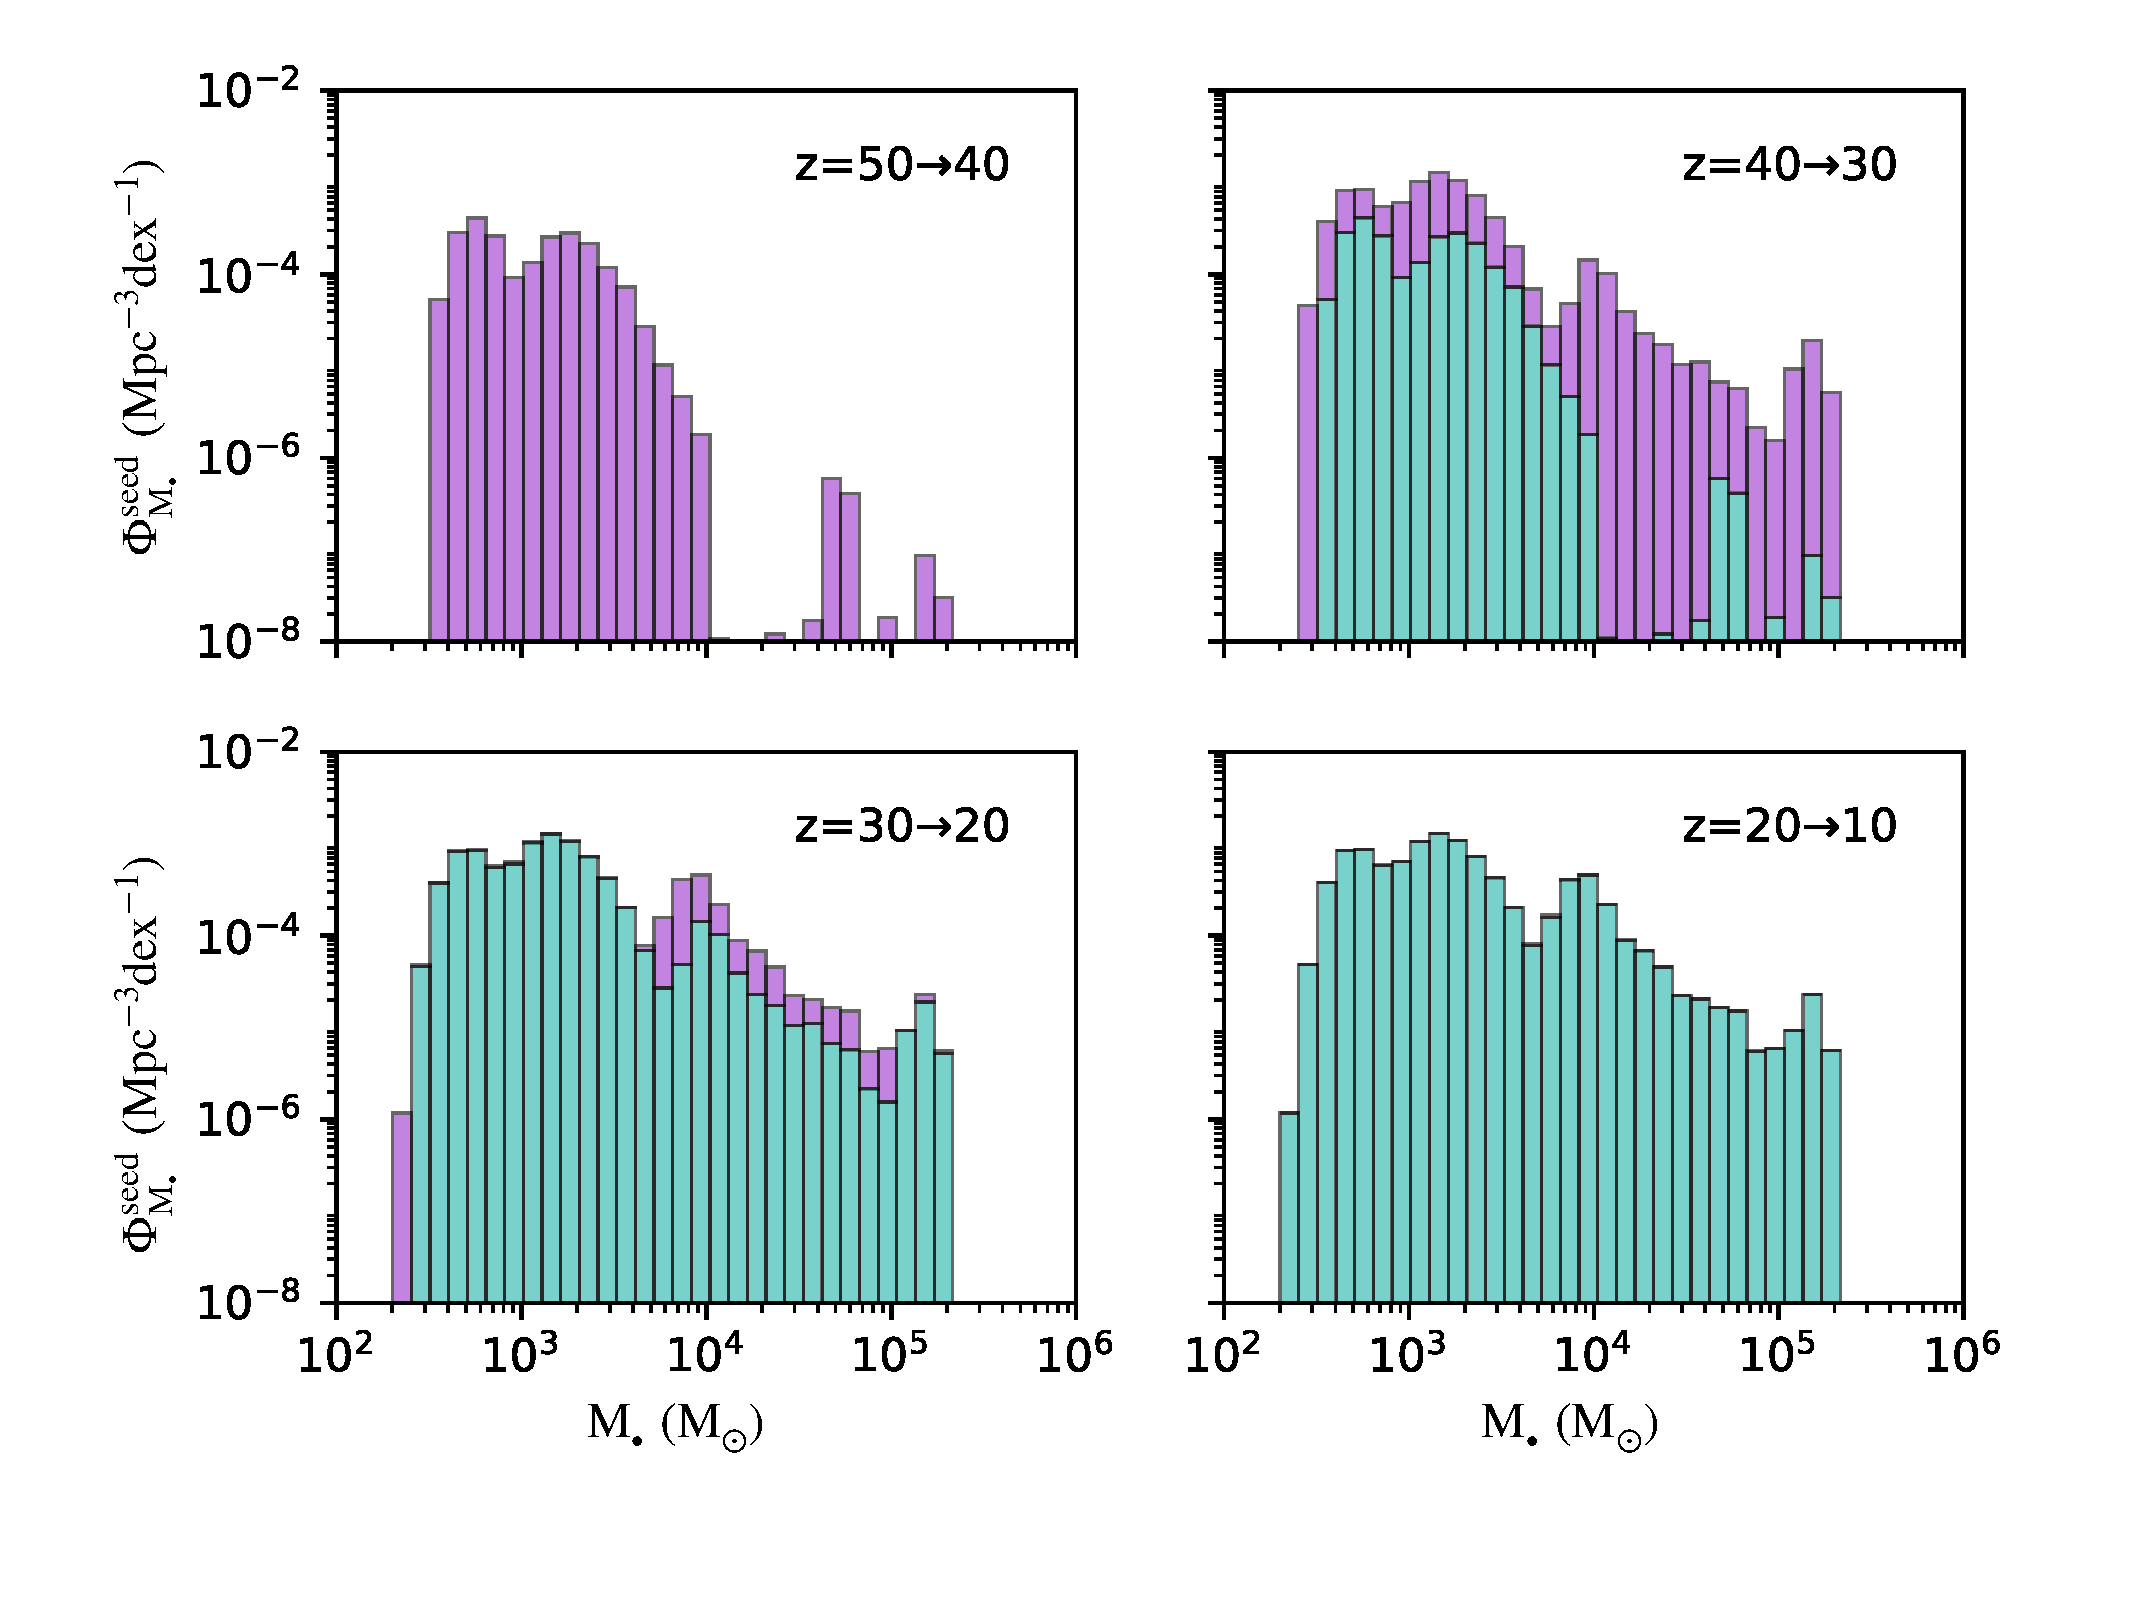
\includegraphics[width=160mm]{seedBHMF_z.pdf}
\caption{
Mass distribution of seed BHs formed in quasar host galaxies at different redshifts ($50\lesssim z \lesssim 10$).
%Each panel includes a redshift span of 10, 
In each panel, the cumulative number distribution of BHs are shown and 
the contribution from newly-born BHs at the redshift interval are denoted with the hatched region.
%with the newly formed BHs denoted by the hatched regions, 
%and the cumulative BHs formed previously by the blue region.
The majority of seed BHs form in the epoch of $40\lesssim z \lesssim 20$.
%The most vigorous seed formation epoches are in redshift ranges $z\sim$ $40-30$ and $30-20$.
Overall, the seed BH mass distribution is extended to $M_\bullet \gtrsim 10^5~\Msun$, 
imprinted with various pathways of parent halo assembly and environmental effects as discussed in \S\ref{sec:seed}.
}
\label{fig:seedmf}
\end{figure*}


Let us consider that a seed BH with a mass of $M_{\bullet,i}$ formed in the $i$-th halo merger tree at the cosmic age $t_i$ ($1\leq i \leq N_{\rm tot}=10^4$),
%In the $i$-th DM growth history where a seed BH is formed with mass $M_\text{itr}$ at the cosmic age $t_\text{itr}$, 
and each of them contributes to the probability distribution function of seed mass at time $t$ as
% 
\begin{equation}
  p^{\rm seed}_i (\Mbh,t)\equiv \frac{\D^2 P^{\rm seed}_i}{\D \Mbh ~\D t}= \frac{ \delta(\Mbh-M_{\bullet,i})~ \delta(t-t_i)}{N_{\rm tot}}.
\end{equation}
%
Based on the cumulative seed mass probability distribution function $\D P^{\rm seed}_i/ \D \Mbh$ 
which is the integral of $p^{\rm seed}_i (\Mbh,t)$ over time, 
we construct the mass function from all $N_{\rm tot}$ seeds formed in one parent halo
with a mass of $\Mh$, where gas has a coherent streaming velocity of $\vbsm$ as a function of time (and redshift).
The absolute abundance of those seed BHs is calculated with the number density of the parent halo in a comoving volume at $z=6$ 
from the Sheth-Tormen mass function \citep{2001MNRAS.323....1S},
%
\begin{align}
  n_{\Mh}= \int_{\Mh}^{10\Mh}  \frac{\D n_{\mathrm{ST}}} {\D \Mh'} \D \Mh', 
\end{align}
%
where we adopt $\Mh = 10^{11}$, $10^{12}$, and $10^{13}~\Msun$, with number densities of
$n_{\Mh} = 9.9\times 10^{-4}$, $6.2\times 10^{-6}$, and $8.9\times 10^{-10}~ \text{Mpc}^{-3}$, respectively.
Combining the PDF and number density normalization, we obtain the seed BH mass function cumulative at time $t$ as
%
\begin{align}
\Phi_{\Mbh}^{\rm seed}\left(t\right) \equiv \sum_{\Mh, \vbsm} n_{\Mh} f_{\vbsm} 
\cdot \sum_{\rm itr} \frac{\D P^{\rm seed}_i}{\D \log \Mbh}\left(t\right) \Big| _{\Mh, \vbsm},
\end{align}
%
where $f_{\vbsm}$ is the volume fraction of the universe with a streaming velocity.
The value is calculated as $f_{\vbsm} = 0.6$ and $0.4$ for $\vbsm = 0$ and $\vbsm=1~\sigma_{\rm bsm}$, respectively. 




%BH seeding is also affected by the baryonic streaming motion of its natal cloud, 
%where gas is streaming relative to the dark matter in the epoch of cosmic recombination at $z_\mathrm{rec}\approx$ 1100, 
%originated from its decoupling with radiation.
%The streaming velocity follows a Maxwell-Boltzmann distribution with a root-mean-square (\textit{rms}) speed of 
%$\sigma(z) = 30~{\rm km~s}^{-1} (1+z)/(1+z_{\mathrm{rec}})$ which is decaying with time \citep{2010PhRvD..82h3520T}.
%The impact of the super-sonic $\vbsm$ at high redshifts on the PopIII star (seed BH) formation 
%is explored by various studies \citep{2012MNRAS.424.1335F,2014MNRAS.439.1092T,2017Sci...357.1375H,2019MNRAS.484.3510S,2021ApJ...917...60L}.
%Their major findings are that the non-negligible $\vbsm$ injects kinetic support into pristine gas clouds, 
%which increases their effective Jeans mass and delays star formation, 
%yielding BH seeds heavier than typical PopIII stars. 
%The volume fraction of the universe with streaming velocities higher than the \textit{rms} value
%is estimated as $\simeq 0.4$. We then set $\vbsm=$ 0 and the \textit{rms} velocity as two representative cases, 
%accounting for roughly $f_{\vbsm} = 60\%$ and $40\%$ of the seeding environments, respectively. 

%%%%%%%
%    Fig. 2
%%%%%%%
\begin{figure*}
\centering
\includegraphics[width=150mm]{scheme.png}
\caption{
Schematical demonstration of the procedure to calculate the evolution of BH mass distribution 
between checkpoints time $t_0$ to $t_0+\tau$. 
The probability of a BH with mass $M_0$ grow to $M$ after $\Delta t=\tau$ is drew from the 
ERDF following Eq.~(\ref{eq:Pl}). 
For a newly formed seed BH $M_{\rm i}$, the probability distribution function of BH mass is a delta function, 
and the growth time is $t_0+\tau-t_{\rm i}$.
Thus the evolution of BH mass distribution is reshaped iteratively 
plus taking account of the newly formed seeds if any.
}
\label{fig:scheme}
\vspace{5mm}
\end{figure*}



% Figure 1 shows the BH seeds formed in progenitors of $\Mh = 10^{11}, 10^{12}$
\vspace{2mm}



\subsection{BH mass growth}
\label{sec:model}
% The BH accretion at high redshifts is probed only by snapshots, in their most luminous quasar phase. 
% We have constraints on simulations and observations of lower redshift counterparts.
With BH seeds planted, we grow the BHs with a semi-analytical accretion rate model and study the evolution of the BH mass distribution until $z=6$. 
\blue{(references + discussion)}
The growth model is characterized by a minimal number of free parameters, 
% the quasar accretion is episodic with Eddington ratio variations,
describing the BH mass growth rate $\Mdot$ by
%%%%%%%
%    Eq. 1
%%%%%%%
% \begin{equation*}
%   \label{eq:mdot_1}
%   \Mdot_\bullet = \frac{\lambda f(\Mbh) \Mbh}{t_{\rm S}} ,
% \end{equation*}
\begin{equation}
  \label{eq:mdot}
  \Mdot_\bullet = \lambda f(\Mbh) \Mdot_\mathrm{Edd} ,
\end{equation}
% where $t_{\rm S} = \eta_0  M c^2/L_{\mathrm{Edd}} \approx 45$ Myr,
where $\lambda \equiv L/L_\mathrm{Edd}$ is the Eddington ratio,
and $\Mdot_\mathrm{Edd} \equiv L_{\mathrm{Edd}}/\eta_0 c^2$ is the Eddington accretion rate with a radiative efficiency of $\eta_0=0.1$ \citep{1973A&A....24..337S},
%Note here we adopt the radiative efficiency $\eta_0 \approx 0.1 $,
%according to the thin accretion disk model \citep{1973A&A....24..337S}, 
which is consistent with the value obtained from the Soltan's argument \citep[e.g.,][]{2002MNRAS.335..965Y,2010ApJ...725..388C}.
% The high mass BH should be strangulated by as it grows, 
\blue{
On the basis of studies on the mass dependence of the radiative efficiency for AGNs at $z\lesssim$ 3 
\citep{2008MNRAS.390..561C,2012ApJ...749..187L,2014ApJ...786..104U}, 
we also introduce a similar functional form which defines the mass dependent function of $f(\Mbh)$ as 
%
\begin{equation}
f(\Mbh) = \frac{2}{1+\left(\Mbh /M_{\bullet,c} \right)^\delta}, 
\end{equation}
%
where we adopt $M_{\bullet,c}=10^8~\Msun$.
With a positive value of $\delta$, the BH growth at the high mass end is suppressed.
%  \blue{(references, Ueda+14?s)}.
}
In the limit of $\delta \ll 1$, where $f(\Mbh) \simeq 1$ is approximated independent of $M_{\bullet,c}$, the model reproduces an exponential growth with an $e$-folding timescale of
$t_{\rm S} =  \Mbh/\Mdot_{\mathrm{Edd}} \approx 45$ Myr, well known as the Salpeter timescale \citep{1964ApJ...140..796S}.
%h independent of BH mass.
% In \S~\ref{sec:fitting}, $\delta$ turns out to be close to 0, indicating an exponential grow manner independent of BH mass.
%Then $t_{\rm S} =  M/\Mdot_{\mathrm{Edd}} \approx 45$ Myr is the Salpeter $e$-folding timescale \citep{1964ApJ...140..796S}.



The quasar activity is episodic in nature, with accretion bursts triggered by gas inflows to the galactic nuclei
% \citep[e.g., mergers or disk instabilities, see][]{2005Natur.433..604D,2005ApJ...630..705H}, 
\citep{2005Natur.433..604D,2005ApJ...630..705H}, 
and the accretion rate declines by self-regulating feedback processes \citep[e.g.,][]{2008ApJ...686..815Y,2011ApJ...737...26N} 
or gas consumption \citep{1991MNRAS.248..754P,2005ApJ...634..901Y,2007MNRAS.377L..25K}. 
This ``flickering'' pattern of individual quasar luminosity evolution can be directly translated into the diversity 
in the Eddington ratios of quasar samples. 
We here suppose that the Eddington ratio distribution function $\D P/ \D\ln\lambda$ (ERDF) is characterized
with a Schechter function and the distribution function is independent of redshift 
\citep{2006ApJ...639..700H,2009ApJ...698.1550H}.
%
For type-I AGN populations at low redshifts, the ERDF is characterized with a Schechter function
%Observations also propose that the intrinsic ERDF in lower-$z$ quasars hosted by star forming galaxies follows a Schechter shape, 
\citep{2015MNRAS.447.2085S,2016ApJ...826...12J,2018MNRAS.474.1225A}.
Motivated by those facts, we give the ERDF by a Schechter function with two free parameters $\lambda_0$ and $\alpha$ as
%%%%%%%
%    Eq. 2
%%%%%%%
\begin{equation}
  \label{eq:Pl}
  \frac{\D P}{ \D \ln \lambda} \propto
  \left(\frac{\lambda} {\lambda_0} \right)^\alpha \exp{\left(-\frac{\lambda}{\lambda_0}\right)}.
\end{equation}
The normalization is set so that the integrant of this function over $\lambda_\mathrm{min}(=0.01) \leq \lambda < \infty$ is unity.
%normalized by the total probability above $\lambda_\mathrm{min}$ = 0.01.
The minimum Eddington ratio $\lambda_\mathrm{min}$ is adopted from the simulated evolution of quasar luminosities 
that decrease mildly toward $\lambda \sim 0.1-0.01$ with $\lesssim$ 100 Myr after the peak activity \citep{2011ApJ...737...26N}.
Moreover, a turnover at the lowest value $\lambda\lesssim 0.01-0.001$ in the ERDF is suggested by observations \citep{2018MNRAS.474.1225A}.  




To characterize the ERDF for a BH population at any time snapshot together with the episodic 
accretion pattern of individual BHs, 
we introduce a time duration of $\tlife$, during which a single value of $\lambda$ that follows 
the ERDF of Eq.~(\ref{eq:Pl}) is assigned to an accreting BH.
In this way, we give a different growth speed of a BH in every period with a duration of $\tlife$ until $z=6$ 
(the corresponding cosmic age is $t_{\rm H}\gtrsim 900$ Myr).
This treatment enables us to capture the nature of accretion bursts and avoid an unrealistically 
long-lasting rapid growth phase of a BH.
This phenomenological method introducing a parameter of $\tlife(<t_{\rm H})$ allows us to avoid 
numerous uncertainties in modeling of the galaxy assembly, gas feeding, and BH feedback processes in the quasar 
progenitor halos.
Instead of treating those ingredients implemented in previous semi-analytical models, we extract 
an averaged but fundamental timescale that governs mutual correlation between the BHMF and QLF,
based on direct comparison to those distribution functions for observed high-$z$ quasar population.
%We leave a more detailed discussion to \S~\ref{sec:discussion}.}


Thus far, we assume that {\it all} the parent halos form seed BHs during their assembly and end up in quasar host galaxies by $z\simeq 6$.
To relax this stringent assumption, we introduce the seeding fraction of $\fseed (\leq 1)$.
As discussed in \citet{2009ApJ...696.1798T}, a small value of $\fseed <1$ is required to avoid overproduction of SMBHs at $z\sim 6$,
depending on BH seeding and growth mechanisms in semi-analytical models.
% that denotes the portion of DM halos where seed BHs are seeded \citep{2009ApJ...696.1798T}.
Since the value has been poorly constrained both by theoretical and observational studies, we treat it as a free parameter.
We take three different values of $\fseed = 1$, $0.1$, and $0.01$ and explore the dependence on the best-fit BHMF and QLF.
Note that the seed mass function shown in Fig.~\ref{fig:seedmf} is given with $\fseed = 1$.



\subsection{BH mass function}\label{sec:MF}

We describe how to calculate the time evolution of the BH mass function, 
combining the semi-analytical growth model and the ERDF (see Eqs.~\ref{eq:mdot} and \ref{eq:Pl}).
We first set a series of checkpoints with an interval of $\tlife$, 
tracing back from $t_{\rm H}(z=6)$ to just prior than the first seed formation time $t_1$, where $t_i$ is the $i$-th seed forming time
as defined in \S\ref{sec:seed} ($1\leq i\leq N_{\rm tot}$).
Note that the number of the checkpoints is given by $\lceil (t_{\rm H}-t_1)/\tau \rceil+1$, where $\lceil x\rceil \equiv {\rm min}\{n \in \mathbb{Z}~ |~x\leq n\}$.
% we set a total number of $\Nt$ checkpoints with an interval of $\tlife$,
% where $\Nt = \lfloor \left(t_\mathrm{H}(z=6) - t_\mathrm{H}(z_\mathrm{seed,max})\right)/ \tlife \rfloor$, 

The time evolution of the BH mass distribution is calculated from the first checkpoint to $t_{\rm H}(z=6)$ by adding newly-forming seed BHs
and taking into account growth of existing BHs via mass accretion.
%every by evolves iteratively during each cycle,together with the seeds newly formed in between.
For a given mass distribution function $\D P/\D  M_{\bullet, 0}$ at a checkpoint of $t=t_0$, 
we give its evolution at $t=t_0+\Delta t$ as
%%%%%%%
%    Eq. 5
%%%%%%%
\begin{equation}
  \label{eq:dpdm}
  \frac{\D P}{\D \Mbh} = \int
   \frac{\D P}{\D \ln \lambda}\Big|_{\lambda_\ast} \cdot
   \frac{\D \ln \lambda_\ast}{\D  \Mbh}\Big|_{\Delta t, M_{\bullet,0}} \cdot
   %_{M, M_\mathrm{i},\Delta t, \delta}
  \frac{\D P}{\D M_{\bullet, 0}}~\D M_{\bullet, 0},
\end{equation}
%
where $\lambda_\ast$ is the Eddington ratio required for a BH with $M_{\bullet,0}$ to grow up to $\Mbh$ within $\Delta t$
and is calculated analytically from Eq.~(\ref{eq:mi2m}) by
%%%%%%%
%    Eq. 4
%%%%%%%
\begin{equation}
  \label{eq:mi2m}
\frac{2 \lambda_\ast \Delta t}{t_{\rm S}}=
  \ln \left(\frac{\Mbh} {M_{\bullet,i}}\right) + \frac{1}{\delta} 
  \left[ \left(\frac{\Mbh}{M_{\bullet,c}}\right)^\delta - \left(\frac{M_{\bullet, 0}}{M_{\bullet,c}}\right)^\delta \right],
\end{equation}
%
with the derivative of ($\D \ln \lambda_\ast / \D  \Mbh )|_{\Delta t, M_{\bullet,0}}$ also determined.
For existing BHs formed prior to this checkpoint, we calculate the evolution of the mass distribution by setting $\Delta t = \tlife$.
% is set for the BH mass distribution iteration from the latest checkpoint, 
For a seed BH formed during this cycle (i.e., $t_0\leq t_k < t_0+\tlife$), 
we evolve $\D P^{\rm seed}_k/\D \Mbh$ by setting $\Delta t = t_0+\tlife -t_k$ and add it to the mass distribution 
of the existing BHs at $t=t_0+\tlife$.
%adopt $\Delta t = t-t_k$, and $\D P^{\rm seed}_{\rm i}/ \D \Mbh$ as the initial mass distribution.
This procedure is illustrated schematically in Fig.~\ref{fig:scheme}. 
% After the seed formation terminates (i.e., after the total number of BHs is fixed), we perform this integration in every timestep 
% by setting to $\Delta t = \tlife$ until $z=6$.
Combining the PDF and number density normalization, the BHMF is given by
%
%%%%%%%
%    Eq. 3
%%%%%%%
\begin{equation}
  \Phi_{\Mbh} 
  =\sum_{\Mh, \vbsm} n_{\Mh} f_{\vbsm} {\fseed} \cdot \frac{\D P}{\D \log \Mbh}\Big|_{\Mh, \vbsm}.
 \end{equation}


To perform the integration and follow the time evolution of the mass function, we set up 
logarithmically spaced mass grids at $10^2 \leq \Mbh /\Msun \leq 10^{12}$.
The number of the grid points is set to $N_{\rm bin}=800$, so that the convergence of the numerical result is ensured.
%
%We note that setting discrete mass bins to resemble the integration in the calculation above, 
%we ensure the convergence of the BHMF produced by increasing the number of mass bins to 800 log evenly across $10^2-10^{12}~\Msun$. 
Our result of $\Phi_{\Mbh}$ is consistent with that obtained from the direct sampling method, where 
we generate $10^7$ BH samples whose initial mass and the Eddington ratio in each cycle are assigned
and reconstruct the BHMF at $z=6$ by collecting the $10^7$ samples.
%Our results of $\Phi_{\Mbh}$ are consistent with that from directly generating random $\lambda$ 
%following Eq.~(\ref{eq:Pl}) in each cycle of BH growth. 
%Remarkably, 
Our method reduces the statistical errors seen in the direct sampling method 
and thus allows us to extend the BHMF and QLF to the higher mass and brighter end
in a reasonable computational time.






% In the BHMF calculation, we set 100 mass bins ranging from  $10^2~\Msun$ to  $10^{12}~\Msun$, spacing evenly in logarithmic scale.
% This enables us to obtain the convergent BHMF at $z=$ 6 for any given parameters.

\vspace{2mm}
\subsection{Quasar luminosity function with obscure correction}\label{sec:LF}

Using the BHMF and its evolution, we construct the QLF, which can be directly probed by high-$z$ quasar observations.
%  compared with observations and in return constrain our model.
For an accreting BH with a bolometric luminosity of $\Lbol=\lambda L_\mathrm{Edd}$, 
its rest-frame ultraviolot (UV) absolute magnitude of $\Muv$ at 1450 $\mathrm{\AA}$ is estimated by
%%%%%%%
%    Eq. 6
%%%%%%%
\begin{equation}
  \label{eq:M1450}
  \Muv= -21.0-2.5 \log  \left(\frac{\Lbol}{10^{45}~\mathrm{erg~s}^{-1}} \right),
\end{equation}
%
where we adopt a bolometric correction factor of $f^{\rm bol}_{1450}=4.4$ for the monochromatic UV band 
\citep{2006ApJS..166..470R}.
Combining this conversion factor and the ERDF to govern the BH growth, the the quasar abundances with different luminosities 
can be constructed straightforwardly.
%Under this conversion, an ERDF combined with the $z\sim$ 6 BH population is able to reproduce 
%the quasar abundances with different luminosities. 
However, we note that the shape and normalization of the {\it intrinsic} QLF is not necessary identical to the {\it observed} QLF
because a larger fraction of fainter quasars are missed in current observations owing to quasar obscuration, 
%it is crucial to obtain we note that a vital ingredient to construct the observed QLF, 
i.e., the number of fainter quasars observed as type-I AGNs is largely reduced by the obscuration effect
%Therefore, is the luminosity dependent obscuration fraction, 
%which decreases the fraction of the detectable quasars preferentially in the dimmer population 
\citep{2003ApJ...598..886U,2014ApJ...786..104U,2008A&A...490..905H,2014MNRAS.437.3550M}. 
%thus differs the normalization and shape of the observed QLF from the intrinsic one.


% 讨论一下 obs fraction 
A widely-accepted mechanism causing quasar obscuration is extinction by dusty tori and dense gas clouds 
in the circumnuclear region, hence tightly related with gas fueling and feedback processes from accreting BHs 
\citep[see][for a review]{2018ARA&A..56..625H}.
However, the physical conditions for quasar obscuration have been poorly understood even with extensive studies both on theoretical and observational sides. 
% our current understanding of the quasar obscured fraction is inadequate, 
%due to the sophisticated physical conditions which lead to obscuration and observational difficulties in probing it.
Observationally, the obscured fraction of AGNs with hydrogen column density of $N_{\rm H}>10^{22}~{\rm cm}^{-2}$
can be estimated from spectral analyses of AGNs in the X-ray band
%The high-$z$ quasars observed in the rest-frame UV-optical bands are profoundly obstructed by dust obscuration, 
%\red{while hard X-rays in the 2$-$10 keV band can penetrate the dust with gas dominating the absorption.} \red{(KI: what does it mean?)} 
%\red{Therefore, dust obscuration is equivalently translated to gas absorption with a hydrogen column density of $N_\mathrm{H}>10^{22}$ cm$^{-2}$ 
%implied by the X-ray spectral fitting 
\citep[e.g.,][]{2003ApJ...598..886U,2007A&A...463...79G,2008A&A...490..905H}. 
The obscured fraction is nearly $\gtrsim 80\%$ at $L_{\rm X}<10^{43}~{\rm erg~s}^{-1}$ and 
decreases with the X-ray luminosity \citep{2014ApJ...786..104U,2014MNRAS.437.3550M}.
The exact function shape still remains under debate, but the overall dependence on the X-ray luminosity holds.
Moreover, the obscured fraction is found to increase gradually toward higher redshifts and is saturated $z\sim 2$
\citep{2008A&A...490..905H,2014ApJ...786..104U,2014MNRAS.437.3550M,2018MNRAS.473.2378V}.


In this work, we adopt the obscuration fraction $\fobsc$ given by \citet{2014ApJ...786..104U}, 
converting the hard X-ray luminosity to the 1450 $\mathrm{\AA}$ magnitude with bolometric correction factors of
\begin{equation*}
  f^{\rm bol}_{\rm X} =
  a\left[1+\left(\frac{\log \left(\Lbol / L_\odot\right)}{b}\right)^{c}\right],
\end{equation*}
where $a=10.96$, $b = 11.93$, and $c = 17.79$ \citep[Eq. 2 in ][]{2020A&A...636A..73D}, 
and $f^{\rm bol}_{1450}=4.4$ \citep{2006ApJS..166..470R}.
The obscuration fraction reads 
\begin{equation*}
  \fobsc = \text{min}\lbrace  0.84 , 0.73-0.24\times[ (\log \Lbol/L_\odot) -43.75] \rbrace,
\end{equation*}
following \citet{2014ApJ...786..104U}.
\blue{
An alternative fitting of $\fobsc$ proposed by \citet{2014MNRAS.437.3550M} 
for their X-ray AGN sample with additional optical obscuration classification gives 
\begin{equation*}
  \fobsc = 0.56 + \frac{1}{\pi} \text{arctan} \frac{43.89 - (\log \Lbol/L_\odot)}{0.46}.
\end{equation*}
We also fit the parameters using this prescription and discuss the sensitivity of results to $\fobsc$ in the Appendix.
}

Here, we neglect the contribution from Compton-thick AGNs with $N_\mathrm{H}>10^{24}$ cm$^{-2}$, 
which are obscured even in the hard X-ray band and show possible dependence on quasar properties.
% and it is currently not warranted to discuss the uncertainties of $\fobsc$.
It is worth noting that the obscured fraction for high-$z$ quasar populations is still under investigation,
and the uncertainties would affect our analyses for fainter quasars.
%with complex conversions between the probes in different observational bands,
% optical and X-ray observations, 
%and is need to be 
%and we may refer to more solid prescriptions of $\fobsc$ in the future.
We leave more comprehensive arguments about the quasar obscuration effect for future work.

After taking into account the obscuration effect, 
the observed QLF for a given BHMF and ERDF is calculated as
%%%%%%%
%    Eq. 7
%%%%%%%
\begin{equation}
\label{eq:dn_dM1450}
\Phi_{\Muv} 
%\equiv \frac{\D n}{\D \Muv} \nonumber \\
 = (1 -\fobsc)  % \nonumber \\
\int \frac{\D P}{\D \ln \lambda}\Big|_{\tilde{\lambda}}  \cdot
\frac{\D \ln \tilde{\lambda}}{\D \Muv} \cdot
 \Phi_{\Mbh} \D \log \Mbh,
\end{equation}
%
where the values of $\tilde{\lambda}=\lambda(\Muv, \Mbh)$ and $\D \ln \tilde{\lambda}/\D \Muv$ are calculated analytically from Eq.~(\ref{eq:M1450}).
%
Hence, the observed QLF can be produced simultaneously with the BHMF from a set of model parameters, 
to be compared with the ones from observation.




\vspace{2mm}
\subsection{MCMC fitting}\label{sec:fitting}

%%%%%%%
%    Fig. 3
%%%%%%%
\begin{figure*}
\centering
\includegraphics[width=180mm]{contour.pdf}
\caption{
Two dimensional posterior distribution of all the model parameters with $\fseed=0.1$ and 0.01, 
along with the marginalized one dimensional projection.
% and the two dimensional distribution between every two parameters. 
The distribution of three parameters ($\tau$, $\lambda_0$, and $\alpha$) show single peaks,
meaning the convergence of those parameters.
The distribution of $\log\delta$ is relatively broader but suggests that the value of $\delta$
is sufficiently low and thus the mass-dependent growth model is excluded.
% confined above the artificial $-3$ barrier, 
%which is sufficiently low and can be neglected in the model.
}
\label{fig:contour}
\vspace{5mm}
\end{figure*}
%


In this section, we describe the Markov Chain Monte Carlo (MCMC) fitting procedure used to optimize 
the BH growth parameters so that the observed BHMF and QLF are consistently reproduced. 
As discussed in \S~\ref{sec:MF}, we consider five parameters of $\tlife$, $\delta$, $\alpha$, $\lambda_0$, and $\fseed$.
The best-fit values of the first four parameters are calculated by the MCMC method, while $\fseed$ is fixed to a single value.
In what follows, we describe the results for $\fseed = 0.1$ and $0.01$ (see Appendix for the case with $\fseed =1.0$).


% prior
In this analysis, we constrain those parameters to be within certain physically acceptable ranges, 
assuming a prior function for each quantity.
We use a uniform prior on $\tlife$ with a limit of $10~{\rm Myr} \leq \tlife \leq 200~{\rm Myr}$,
motivated by the constraints on the quasar lifetime based on various observations
\citep[e.g.,][]{2004cbhg.symp..169M}.
The parameter of $\delta$ that characterizes a non-exponential BH growth 
is constrained at $\log \delta$ from $-4$ to $-0.3$ 
\footnote[2]{ We first set uniform prior $0\leq \delta \leq 1$, 
and find the posterior distribution assembles to $\delta \lesssim 0.1$.
We then switch to impose the $\log \delta$ prior to improve the fitting performance at small $\delta$ values.
}, 
\red{KI: add a footnote, explaining why not $\delta$ but $\log \delta$?}.
%slightly suppressing the growth in the high mass end. 
% After trials we find in the Markov chain, the value of $\tlife$ reduces to $\lesssim$ 100 Myr, 
% and the one for $\delta$ assembles to $\lesssim 0.1$. 
% Driven by these phenomena, we switch the uniform $\tlife$ prior to 10 to 200 Myr,
% and use $\log \delta$ instead of $\delta$ with a prior ranging from $-4$ to $-1$ in pursuit of better fitting performance. 
The prior function is uniform at $\log \delta \geq -3$ and is imposed to decay with an exponential cutoff at $\log \delta < -3$,
which is small enough for the model to be approximately mass independent.
%since toward low $\log\delta$ the model is essentially mass-independent,
%and remains uniform otherwise. 
For the characteristic Eddington ratio $\lambda_0$ in the Schechter-type ERDF, 
we impose a Gaussian prior function with a mean value of $\mu_{\lambda_0}=0.6$ and a dispersion of $\sigma_{\lambda_0}=0.4$.
% motivated by the various observations revealing a large sample of quasars with peak $\lambda\lesssim 1$,
The choice is motivated by the brightest quasar samples at $z=$ 6, whose ERDF function is peaked around $\lambda \sim 0.6$ 
% \citep[e.g.,][Onoue et al. in preparation]{2010AJ....140..546W}.
\citep[e.g.,][]{2010AJ....140..546W}.
\red{Specially a complete sample of quasars from Onoue et al. in prep peak with $\log \lambda_0 \approx -0.24 \pm 0.31$ 
before correcting the selection bias. (to be revised by MO)}.
% It is worth noting that, observationally the high-$z$ ERDF is fitted by a log-normal function. 
% \blue{
% because of detection limit, there may be a large population of low $\lambda$ BHs unrevealed,
% so our model of Schechter distribution is purely from theoretical prediction 
% and extrapolation of the statistical properties of its low-$z$ counterparts. 
% Then the slope index alpha uncertain \dots
% }
% However, lower-$z$ quasar observations reveal that ERDF is better fitted by a Schechter function \citep{2015MNRAS.447.2085S}, 
% indicating a prominent population of low $\lambda$ quasars is hidden by the flux-limited incompleteness.
For the low-$\lambda$ slope of $\alpha$ in the ERDF, we assign a Gaussian prior function with a mean value 
$\mu_{\alpha}=0$ and a dispersion of $\sigma_{\alpha}=0.3$.
Note that the value of $\alpha$ remains poorly constrained by the current high-$z$ quasar observations,
but the low-$z$ quasar samples support $-0.3 \lesssim \alpha \lesssim 0.3$ \citep[e.g., see Figure 21 in][]{2015MNRAS.447.2085S}.
% considering the more significant obscuration of lower $\lambda$ quasars 
%we assign a Gaussian prior, with the mean value $\mu_{\alpha}=0.$ and scatter $\sigma_{\alpha}=0.3$.


%
% 1. data: observational MF LF; describe quadratic error in Willott 2010
The observed BHMF data is taken from \citet{2010AJ....140..546W} (hereafter \citetalias{2010AJ....140..546W}), where 
the virial BH mass measurements for $\sim 20$ bright quasars at $z\simeq $ 6 are used.
%rom the virial BH mass among $\sim$ 20 quasars at $z\approx$ 6.
%they reconstruct the BHMF with the QLF and ERDF
%extracted from the virial BH mass among $\sim$ 20 quasars at $z\approx$ 6. 
Although the BHMF spans over $10^7 < \Mbh/\Msun <10^{10}$, the best constraint is given around 
$\Mbh \simeq 10^{8.5}~\Msun$
and thus the statistical error size becomes larger both at the lower and higher mass range.
We set up 10 logarithmically spaced mass bins and adopt errors with sizes increasing quadratically as 
$\Phi_{\Mbh}^{\rm err} = \pm \{0.2 +   [\log (\Mbh/10^{8.5}~\Msun)]^2/3 \}~{\rm dex}$,
covering the same mass range as in their bootstrap resamples (see Figure 8 of W10). 
The observed QLF is taken from \citet{2018ApJ...869..150M} (hereafter \citetalias{2018ApJ...869..150M}) 
over a wide range of $-30 < \Muv <-22$ mag (see their Table 4 and Figure 13). 
The magnitude bins and the error sizes are given consistently with \citetalias{2018ApJ...869..150M}.

  

% 3. posterior
% Then evaluating the likelihood of the dataset reproducing the observed BHMF and QLF at $z=$ 6, 
% the Markov chain of samples converges to the best-fit (maximum likelihood) parameters.
Following the prior distribution functions, the four parameters are sampled to generate the synthetic 
BHMF and QLF dataset, which are compared to the observational dataset. 
The discrepancy between the model and observational data is evaluated with a $\chi^2$-value defined by
%%%%%%%
%    Eq. 8
%%%%%%%
\begin{align}
  \chi^2 = \sum_{i,j}
  \frac{\left(\log{\Phi^{\rm mod}_{i,j}} - \log{\Phi^{\rm obs}_{i,j}}\right)^2}{(\log{\Phi^{\rm err}_{i,j}})^2},
\end{align}
where $\Phi^{\rm mod}_{i,j}$ and $\Phi^{\rm obs}_{i,j}$ represent the modeled and observational value 
on the \textit{i-}th BHMF ($j=\Mbh$) and QLF ($j=\Muv$) bin, and $\Phi^{\rm err}_{i,j}$ is the corresponding error.
Adopting 10 mass bins and 12 magnitude bins, we treat the errors from comparison both in the BHMF and QLF
with a nearly equal weight.
%te that the equal constraints from the BHMF and QLF are realized by extracting
%comparable numbers of data points from $\Phi_\mathrm{M}$ and $\Phi_\mathrm{\Muv}$.
% the constraint is actually insensitive to the choice of bin numbers. 
The posterior distribution of the MCMC fitting is stabilized around the minimum value of $\chi^2$ (highest likelihood), 
with the models best reproducing the $z=$ 6 BHMF and QLF.



\vspace{5mm}
\section{Results}\label{sec:result}


%%%%%%%
%    Fig. 4
%%%%%%%
\begin{figure*}
\centering
\includegraphics[width=160mm]{fits_MF.png}
\caption{
The BH mass function at $z=6$ with the best-fit parameters (purple curve) and the $1\sigma$ spread for the cases with $\fseed=0.1$ (left) and $0.01$ (right). 
For comparison, the BHMF inferred by \citetalias{2010AJ....140..546W} is overlaid (blue curve and shaded region).
The data is used for the model parameter fitting.
%.The blue line shows the BHMF derived by \citet{2010AJ....140..546W}.
% error of observation
}
\label{fig:fitmf}
\end{figure*}


%%%%%%%
%    Fig. 5
%%%%%%%
\begin{figure*}
\centering
\includegraphics[width=160mm]{fits_LF.png}
\caption{
The quasar luminosity function at $z=6$ with the best-fit parameters (purple curve) and the $1\sigma$ spread for the cases with $\fseed=0.1$ (left) and $0.01$ (right). 
%as described in \ref{fig:fitmf}. 
The observed data (blue symbols) with error bars are taken from \citetalias{2018ApJ...869..150M} and is used for the model parameter fitting.
}
\label{fig:fitlf}
\end{figure*}



\vspace{2mm}
\subsection{Fitting Results}\label{sec:fitting_result}
In Fig.~\ref{fig:contour}, we visualize the MCMC fitting results for each parameter in two-dimensional 
posterior distribution for the case $\fseed= 0.1$ (left) and $0.01$ (right), respectively.
The three vertical lines on each one-dimensional posterior distribution present the peak and the values
with $1\sigma$ scatter.
The result for the $\fseed=1$ case is discussed in the Appendix.


For the two cases, the best-fit solutions consistently show a small values of $\delta < 0.01$.
%, which is sufficiently small and should be marginalized out. 
This suggests that in our model assumption, a nearly exponential BH growth pattern is favored. 
% In other words, on average the BH growth can be described as exponential, 
% under the premise that the gas supply is episodical. 
The typical duration of quasar activity is required to be $\tlife \simeq 29$ Myr for both the cases, 
which is $\sim 64\%$ of the $e$-folding time for an exponential growth.
This suggests that accreting seed BHs vary their growth speeds (i.e., the Eddington ratio) 
$\sim 30$ times on average, toward the cosmic time of $t_{\rm H} \gtrsim 900$ Myr at $z\simeq 6$.
The timescale of $\tlife$ also gives a lower bound of the quasar lifetimes of $t_{\rm Q}\sim 1-10$ Myr, 
which are estimated by the measurement of the physical extents of hydrogen Ly$\alpha$ proximity zones 
observed in the rest-frame UV spectra (e.g., Eilers+2018, Davies+ 2019).\red{KI: we need to figure out 
if their $t_Q$ is the quasar age or lifetime, or something else?}
More detailed comparison is discussed in \S\ref{sec:evol}.


%%%%%%%
%    Fig. 
%%%%%%%
\begin{figure*}
\centering
\includegraphics[width=160mm]{tau.png}
\caption{
Left panel: BHMF at $z=$ 6 calculated in the $\fseed=0.01$ case, 
with different $\tlife=$ 10, 18 (the best-fit value), and 50 Myr, respectively, 
and other parameters are fixed to the best-fit values. 
The blue curve denotes the BHMF constrained by the \citetalias{2010AJ....140..546W} result. 
With lower(higher) $\tlife$ than the best-fit value, the BHMF is under(over)-produced in the high mass end.
Right panel: QLF at $z=$ 6 calculated with the same parameters as in the left panel.
The overlaid blue dots are from the \citetalias{2018ApJ...869..150M} $z\sim$ 6 quasar observation. 
With $\tlife$ values different from the best-fit value, the consequent QLF show 
similar trends of deviation from observation as in the BHMF curves.
}
\label{fig:tau}
\end{figure*}


The two parameters characterizing the ERDF are given as
$(\lambda_0,\alpha) = (0.89,0.12)$ and $(0.87,0.20)$ for $\fseed=0.01$ and $0.1$, respectively.
\blue{
With those values, the number fraction of super-Eddington accreting BHs is
estimated as $P(\lambda>1)=0.064$ and 0.075, respectively. 
The small discrepancy is enlarged with the multiple cycles of assigning $\lambda$ to BH growth, 
and increase the fraction of the super-Eddington phase for smaller $\fseed$. 
Thus for different $\fseed$ values, a similar number density of BHs which rapidly grow to be SMBHs by $z\simeq 6$ is produced, 
consistent with a general picture for the early assembly of SMBHs 
\citep[e.g.,][]{2006NewAR..50..665F,2008AJ....135.1057J,2010AJ....139..906W}.
The characteristic Eddington ratio needs to be close to unity, otherwise the highest luminosity and BH mass
in the model would differ from those in observations.
On the other hand, the power-law index of $\alpha$ in the ERDF tends to increase as the seeding fraction decreases,
indicating that fraction of active BHs with $\lambda \gtrsim 1$ is elevated. 
Thus, with lower seeding fractions, the high-$z$ quasar assembly spends a larger fraction of time in active phases 
and reproduce the bulk properties of the BHMF and QLF.
}


In Figs.~\ref{fig:fitmf} and \ref{fig:fitlf}, we show the BHMF and QLF at $z=$ 6 reproduced by the best-fit parameters
as well as the $1\sigma$ spread, where the QLF model excludes a contribution from obscured quasars, 
yielding the {\it observed} QLF for type-I AGN populations.
The observed BHMF in \citetalias{2010AJ....140..546W} and QLF in \citetalias{2018ApJ...869..150M} 
with statistical errors are also overlaid for comparison.
We note that \citetalias{2010AJ....140..546W} constructed the BHMF using quasar samples with 
$10^8~\Msun \lesssim \Mbh \lesssim 3\times 10^9~\Msun$.
In the high-mass regime, our fitting result nicely agrees to that in \citetalias{2010AJ....140..546W}.
The QLF fitting results are also consistent with the observed one over $-29~{\rm mag} \lesssim \Muv \lesssim -25~{\rm mag}$,
but seems to overproduce the abundance of fainter quasars at $\Muv>-24~{\rm mag}$.
% due to the lack of fine tuning by the model parameters in the low mass range, 
The difference at the fainter end tends to be alleviated with the seeding fraction lowered ($\fseed = 0.01$),
because the progenitors of $z=6$ BHs with $10^{7-8}~\Msun$ (or similarly, 
$-22~{\rm mag} \lesssim \Muv \lesssim -24~{\rm mag}$) were less massive seed BHs with $\sim 10^4~\Msun$,
which is closer to the peak of the seed mass distribution (see Fig.~\ref{fig:seedmf}).
Those BH population naturally produces a flatter slope of the QLF (and BHMF) at the faint (low-mass) end.
Overall, the parameters are inferred to be reasonable fits consistent with the observational data.



\vspace{2mm}
\subsection{Model dependence}\label{sec:modep}
As described in \S~\ref{sec:model}, we introduce the parameter $\tau$ as a typical timescale
for individual durations of quasar accretion activity.
Specifically, we assign an Eddington ratio $\lambda$ following the ERDF for all BHs in each cycle
with a time duration of $\tau$.
Variable accretion episodes in every cycle essentially modify the effective ERDF in the whole BH growth history,
because multiple sampling of $\lambda$ reduces the possibility of a BH growing with $\lambda \gtrsim \lambda_0$
compared to that with a single sampling of $\lambda$.
%However at any time during growth, the ERDF of the BH population remains the same as at $z\sim$ 6,
%therefore we ensure treating all cosmic time equally.
In what follows, we demonstrate the role of $\tlife$ in shaping the BHMF evolution and the consequent QLF.
% tau极端小,则非常小的lambda,不能解释 (且delta func? 有必要说或是放在后面讨论?)

In the left panel of Fig.~\ref{fig:tau}, we present the BHMF at $z=6$ for three different values of $\tlife=10$, $18$, and $50$ Myr,
but keeping the other parameters as the best-fit values ($\lambda_0=0.87$ and $\alpha=0.20$) for the case with $\fseed=0.01$.
We note that $\tlife \approx$ 18 Myr is the best-fit value reproducing the BHMF consistent with that of \citetalias{2010AJ....140..546W}.
%the other two cases demonstrate the sensitivity of the $\tlife$ value in producing the bulk of massive BHs
%and the slope in the high mass tail.
For $\tlife=10$ Myr, the frequency of Eddington ratio assignment increases twice until $z=6$.
%to $\sim$ 80 from $\sim$ 40 with the best-fit $\tlife$ value.
Therefore, continuous and efficient growth of BHs with $\lambda \gtrsim \lambda_0$ is less likely to occur,
%high Eddington ratio accretion along the growth is lower,
suppressing the formation of BHs heavier than $M_\bullet \simeq 10^8~\Msun$.
Moreover, if a high Eddington ratio is given with a certain but low probability, the BH mass hardly increases
within $\tlife=10$ Myr, which is $\simeq 20\%$ of the $e$-folding timescale.
On the other hand, for $\tlife=$ 50 Myr, there is a non-negligible probability that
% $\sim$ 16 times of Eddington ratio assignment,
more BHs experience high accretion rates with $\lambda\gtrsim \lambda_0$ through their assembly history.
%high values of $\lambda\gtrsim \lambda_0$ is non-negligibly realized in the BHMF evolution.
Therefore, the high mass end of the BHMF is further extended and those massive populations are substantially
overproduced compared to the observed abundance.
%in the high mass end of BHMF at $z=$ 6, the BH population is significantly overproduced than the constraints from observation.

The QLF at $z=6$ is shown in the right panel of Fig.~\ref{fig:tau}.
%In the conversion from BHMF to QLF, the ERDF is the same for different $\tlife$ values,
%following the $P(\lambda)$ in Eq.~(\ref{eq:Pl}) with $\lambda_0=0.87$ and $\alpha=0.20$.
Overall, the dependence of the QLF on the choice of $\tau$ shows the same trend as in the BHMF,
%the deviation from the observed QLF of \citetalias{2018ApJ...869..150M} shows similar trends as in the BHMF.
i.e., higher (lower) $\tlife$ values lead to under(over)-production of the luminous quasar population.
The best-fit value of $\tlife (\simeq 18$ Myr) favors a moderate fraction of $t_{\rm S}$.
This suggests the importance of regulated growth of BHs to reproduce the shape of the observed BHMF and QLF.
%reproduces the quasar observation together with the other best-fit parameters in their reasonable ranges.
In \S\ref{sec:evol}, we apply this episodic accretion model to individual growth pathways of high-$z$ quasars
and demonstrate that normal seeding mechanisms can explain the existence of massive BHs with low luminosity
observed at $z\simeq 6-7$.

\vspace{2mm}
\section{Cosmological evolution of BH mass and quasar luminosity function}\label{sec:cosm}
%\red{KI: shall we discuss the $z$-dependence of the BHMF and QLF?
%Don't need to repeat calculations. Just using the same parameters with 1sigma scatter?
%Showing $\rho_{\bullet}(z)$ in $\Msun ~ {\rm Mpc}^{-3}$, which is the integrant of BHMF, would be interesting}


%%%%%%%
%    Fig. 
%%%%%%%
\begin{figure*}
\centering
\includegraphics[width=160mm]{BHMF_rhoz.png}
\caption{
{\it Left panel}: BH mass functions at different redshifts of $6\leq z \leq 10$.
The solid lines denote modeled BHMF produced by the best-fit parameters 
and the shaded regions present the $1\sigma$ spread. 
{\it Right panel}: the redshift evolution of the cumulative mass density of BHs with $\Mbh \geq 10^7~\Msun$ in a comoving volume, 
evaluated by the integration of the BHMF shown in the left panel.
The evolutionary trend can be approximated as $\rho_\bullet (z) \propto 10^{k_M z}$, where $k_M\simeq -0.8$.
}
\label{fig:BHMF_rhoz}
\end{figure*}


\begin{table}
\renewcommand\thetable{1} %! fix indexing
\caption{$\rho_\bullet(z)$ Evolution Parameters}
\begin{center}
% \tablenum{1}
\begin{tabular}{l c r}
\hline
$M_{\rm min}$ & $\log \rho_{\bullet,0}$ & $k_{\rm M}$ ~~~ \\ 
\hline 
\hline
10$^7$  &  $-5.91\pm 0.28$  &  $-0.58 \pm 0.21$  \\
10$^8$  &  $-6.93\pm 0.47$  &  $-0.78 \pm 0.31$  \\
% 10$^9$  &  $-8.30_{-0.47}^{+0.47}$  & $-1.04_{-0.58}^{+0.54}$ \\
10$^9$  &  $-8.30\pm 0.47$  &  $-1.04 \pm 0.58$ \\
\hline 
\end{tabular}
\label{tab:MFz}
\end{center}
\end{table}  

Based on the constraint from $z\sim 6$ quasar observations, the best-fit model from the MCMC realizations enables
us to probe the statistical BH evolution at higher redshifts.
As a fiducial case, we take the best-fit parameters of BH growth for $\fseed=$ 0.01,
where $\tlife=18.76$ Myr, $\delta=0.055$, $\lambda_0=0.87$, and $\alpha=0.20$.
We apply the result to construction of BHMFs and QLFs at higher redshifts and give implications for
the future explorations of high-$z$ quasars.



\subsection{Black hole mass function}

In the left panel of Fig.~\ref{fig:BHMF_rhoz}, we show the BHMFs at five different redshifts of $z=6-10$.
For all the redshifts, the BHMFs can be characterized with a double power-law function, similar to lower-$z$ quasar populations.
From higher to lower redshifts, the number density of BHs heavier than $M_\bullet = 10^7~\Msun$ increases
and the high-mass tail of the distribution is extended owing to efficient growth of the most massive BH population.
%The number density of BHs with $\Mbh=10^7~\Msun$ emerging from high redshifts increase by a factor of $\sim 4$ per unit redshift.
In the right panel of Fig.~\ref{fig:BHMF_rhoz}, we also present the cumulative mass density of BHs with $\Mbh \geq M_{\rm min}$ in a comoving volume,
defined by the integration of the BHMF as
%
\begin{equation}
 \rho_\bullet(z)=\int_{M_{\rm min}}^{\infty} \Phi_{\Mbh} (z) \Mbh \D \log \Mbh,
\end{equation}
%
%as a function of redshift.
where we set the minimum mass to $M_{\rm min}=10^7$, $10^8$, and $10^9~\Msun$.
This result shows that the early BH assembly takes place rapidly and the redshift-dependence can be approximated by
%
\begin{equation}
\rho_\bullet(z)
%= \rho_{\bullet 0}\cdot e^{k_{\rm M}(z-6)}
\simeq \rho_{\bullet,0}~ 10^{k_{\rm M}(z-6)},
\end{equation}
%
where the fitted values of $\rho_{\bullet,0}$ and $k_{\rm M}$ are shown in Table.~\ref{tab:MFz}.
On the other hand, the stellar mass density of the quasar progenitor halos is calculated as
%
\begin{equation}
\rho_{\star}(z)
\simeq f_\star n_{\Mh} M_h~ 10^{k_{\rm h}(z-6)},
\end{equation}
%
where $f_\star(\equiv M_\star/\Mh)$ is the mass ratio of the galaxy stellar mass to the DM halo mass and
$n_{\Mh}$ is the number density of quasar host halos with $\Mh$ in a comoving volume at $z=6$; namely,
the value of $n_{\Mh}\Mh \simeq (6.2-99)\times 10^6~\Msun~{\rm Mpc}^{-3}$.
We here express the mass growth of the DM halo with a functional form of $\propto 10^{k_{\rm h} z}$,
which nicely reproduces the mass growth of DM halos
\citep[e.g.,][]{2002ApJ...568...52W,2008MNRAS.383..615N,2008MNRAS.388.1792N,2010MNRAS.406.2267F}
\footnote[3]{
In fact, this redshift dependence leads to a halo-mass growth rate of $\D \left(\ln \Mh \right) / \D t \propto(1+z)^{5/2}$,
which has been understood based on the extended Press-Schechter formalism and also derived by
a fit to merger trees from cosmological N-body simulations \citep{2013MNRAS.435..999D}.}.
% The redshift dependence yields the cosmic BH growth rate in the matter-dominated universe
% as $\dot{\rho}_\bullet \propto \rho_\bullet (1+z)^{5/2}$ or

% \begin{align}
% \dot{\rho}_\bullet(z) & =\dot{\rho}_\bullet(z=6)\left(\frac{1+z}{7}\right)^{5/2} 10^{k_{\rm M}(z-6)}, \\
% &\simeq *** ~\Msunyr~{\rm Mpc}^{-3} \left(\frac{1+z}{7}\right)^{5/2} e^{\bar{k}_{\rm M}(z-6)},\nonumber
% \end{align}

% where $\bar{k}_{\rm M} \equiv k_{\rm M} \ln 10 \simeq -1.84$.
% \red{KI: I'm not sure what we discuss here... One thing is the cosmic SFR density (Madau's plot).
% Is there something like Madau's plot but for DM halos?}
% The exponential dependence on redshift is reminiscent of the cosmic galaxy mass growth
% $M_{\star} \propto e^{-B z}$, as a consequnce of the assumption of fixed galaxy to DM halo mass ratio,
% and the growth rate of DM halos in the extended Press-Schechter formalism
% $\D \left(\ln \Mh \right) / \D t \propto(1+z)^{5/2}$ \citep{2008MNRAS.383..615N}.
% Our results suggest that the cumulative massive BH mass density growing in galactic nuclei also follows
% an exponential evolution with redshift,
% which is statistically in agreement with the host halo and galaxy growth.
The star-to-halo mass ratio is assumed to be $f_\star =0.01$ for those quasar progenitor halos at $z>6$
% (UNIVERSEMACHINE; Behroozi et al. 2019).
\citep[fits by code {\tt UNIVERSEMACHINE} in][]{2019MNRAS.488.3143B}.
%https://ui.adsabs.harvard.edu/abs/2019MNRAS.488.3143B/abstract
With those values, we estimate the stellar-to-BH mass ratio for high-$z$ quasars as
%
\begin{equation}
\frac{\rho_{\star}(z)}{\rho_{\bullet}(z)}
\simeq 2.5\times 10^{3} \left(\frac{f_\star}{0.01}\right)
~ 10^{(k_{\rm h}-k_{\rm M})(z-6)},
\end{equation}
% 
\red{KI: please check the value of $k_{\rm h}-k_{\rm M}$.}
\blue{
where $k_{\rm h} \approx -0.16 $ for the parent halo growth histories.
}
Therefore, at $z\sim 6$ the bulge-to-BH mass ratio $\sim O(10^3)$ for the entire BH population (i.e., low-mass BHs and low-luminosity quasars) 
is broadly consistent with those seen in the local universe, although SMBHs observed as high-$z$ quasars
appear to be overmassive compared to the local relation \citep[e.g.,][]{2013ApJ...773...44W,2020A&A...637A..84P}.



\subsection{Quasar luminosity function}

Next, we show the QLFs at different redshifts of $z=6-10$ taken from the BH growth model in the left panel of Fig.~\ref{fig:QLF_rhoz}.
%The model QLFs we propose give interesting prediction and will be further constrained by higher redshift quasar observations.
\red{KI: add more explanations about the QLFs. How about the detection limits of Euclid, Roman, and others?
Also, you could compare your results with Aaron Yung's results.}
In the right panel of Fig.~\ref{fig:QLF_rhoz}, we present the number density of luminous quasars with $\Muv <-26$ as a function of redshift.
The evolutionary trend can be fitted as $\propto 10^{k_{\rm L}z}$, where $k_{\rm L}\approx -0.97$.
A rapid decay of the quasar number density toward higher redshifts is found by previous studies \citep[e.g.,][]{2001AJ....122.2833F,2016ApJ...833..222J},
which show $k_{\rm L}= -0.47$ and $-0.72$ from the analysis of quasar samples at $z\simeq 3-5$ and $z\simeq 5-6$, respectively.
Recently, a steeper decline of luminous quasar number density toward higher redshifts is proposed by \citet{2019ApJ...884...30W},
suggesting $k_{\rm L}=-0.78$ at $6\lesssim z \lesssim 7$.
%a steeper decline ifts is suggested in recent studies of $z\gtrsim 6$ quasars,
%e.g. \citet{2019ApJ...884...30W} measure the spatial density of $z\sim 6.7$ quasars,
%and fit the parameter $k_{\rm L}=-0.78$ by connecting the $z\sim 6$ result from \citet{2016ApJ...833..222J}.
The rapid decline toward higher redshifts is nicely characterized by the treatment of episodic natures of BH accretion with a finite value of
$\tau ~(\simeq 20~{\rm Myr})$, in order to match the statistical properties of high-$z$ quasars.
We also note that the tendency would be explained by the rarity of massive quasar-host halos at higher redshifts,
non-constant radiative efficiencies that covert the BH growth rate into the luminosity, or some combination of these effects
\citep[e.g.,][]{2010ApJ...718..231S}.
%Studies with the assumption of the close correlation of DM halo mass with central BH mass, and a constant Eddington ratio 
%interprete this rapid decline by the rarity of massive halos toward higher redshifts \citep[e.g.,][]{2010ApJ...718..231S}, 
%while another entangling factor is the radiative efficiency in converting BH growth rate to luminosity. 
%In our work, we argue that the episodical BH accretion with bursts and quiescent phases is 
%important in matching the $z\sim 6$ quasar observations, 
%and this calls consideration of the more realistic BH-galaxy coevolution in understanding the observable AGN properties.


%%%%%%%
%    Fig. 
%%%%%%%
\begin{figure*}
\centering
\includegraphics[width=160mm]{QLF_rhoz.png}
\caption{
{\it Left panel}: quasar luminosity functions at different redshifts of $6\leq z \leq 10$. 
The solid lines denote modeled QLF produced by the best-fit parameters and the shaded regions present the $1\sigma$ spread. 
{\it Right panel}: the redshift evolution of the cumulative number density of quasars with $\Muv <-26~{\rm mag}$ in a comoving volume,
evaluated by the integration of the QLF shown in the left panel.
The evolutionary trend can be approximated as $n(\Muv<-26~{\rm mag})\propto 10^{k_{L} z}$, where $k_L \simeq -0.95$.
This result indicates rapid decline of the number of bright quasars toward higher redshifts, consistent with previous observations
\citep[red data points; see][]{2016ApJ...833..222J, 2019ApJ...884...30W}
}
\label{fig:QLF_rhoz}
\end{figure*}



\section{Discussion}
\label{sec:discussion}
\vspace{2mm}
\subsection{Individual BH growth}\label{sec:evol}

From the BH growth model described in \S~\ref{sec:MF}, we further explore individual BH evolutionary tracks starting from the BH seeds.
% We take $\fseed=$ 0.01 as a fiducial case, where the best-fit parameters for BH growth are 
% $\tlife=18.76$ Myr, $\delta=0.055$, $\lambda_0=0.87$, and $\alpha=0.20$.
% We apply the result to construct individual evolutionary tracks of BHs and produce implications to high-$z$ quasar observations.
% We generate a 10$^7$ sample of BHs at $z=$ 35, with seed mass $M_\star = 1.5\times 10^3~\Msun$, 
% \blue{(10$^5$ sample size actually, but with $\fseed=0.01$, essentially 10$^7$)}
% \blue{(1e3 $\Msun$ in plot, with seed mass and redshift distribution can also be realized)}, 
% motivated by the properties of typical BH seeds (with median formation redshift and median mass).
We generate a sample of 10$^7$ BHs, whose formation time and mass distribution at birth follow the model described in \S~\ref{sec:seed}. 
Following the best fit parameters in the case of $\fseed = 0.01$,
we assign an Eddington ratio $\lambda$ in every interval $\tlife=18.76$ Myr to grow the individual BHs until $z=6$. 
The value of $\lambda$ follows the ERDF characterized by a Schechter distribution with $\lambda_0=0.87$ and $\alpha=0.20$.
With those parameters, we show the BH growth tracks that end up with $>10^8~\Msun$ by $z=6$ in Fig.~\ref{fig:track}. 
\red{KI: what is the frequency $N$ of BH accretion bursts with $\lambda>\lambda_0$ between $z=6$ and $10$? The duty cycle for the sub-sample
is $f_{\rm duty}\simeq N\tlife/\Delta t_{\rm H}$.}
\blue{
We take this sub-sample representing the observable massive BH population,
which is easier to be probed by flux-limited quasar observations.
During the growth histories of these BHs, it is interesting to examine the duty cycle of the active phase, 
e.g., characterized as $f_{\rm duty}\simeq N\tlife/\Delta t_{\rm H}$,
where $N$ is the frequency of a BH growing with super-Eddington accretion bursts,
in a time duration $\Delta t_{\rm H}$.
We estimate the duty cycle between the cosmic age of $z=$ 10 to $z=$ 6,
and find $f_{\rm duty}\simeq 0.15$.
On the other hand, the value of $f_{\rm duty}$ in the whole BH population 
can be estimated as the probability of super-Eddington realization in one single epoch 
$P(\lambda>1)=$ 0.075 (see \S~\ref{sec:fitting_result}), 
which is about twice lower than the value of $f_{\rm duty}$.
Therefore the massive sub-sample is biased toward the BHs undergoing more active accretion episodes.
}

In this sub-sample, we find seven BHs heavier than $M=10^9~\Msun$ (highlighted with solid curves), 
among which five BHs show $\lambda<1$ in the snapshots at $z=6$.
Tracing the BH growth curve back to $z=30$ with the Eddington ratio observed at $z=6$ (dotted curves),
the extrapolated mass of those sub-Eddington BHs at $z=6$ is as massive as $\Mbh \gg 10^5~\Msun$ and is 
substantially higher than the mass range for seed BHs.
%ting BHs trace back to exceedingly massive seeds which are hard to be explained by current seeding scenarios. 
%
%If we extrapolate the BH mass with the $z \sim$ 6 witnessed Eddington ratio back to $z\sim$ 30, 
%the sub-Eddington accreting BHs trace back to exceedingly massive seeds which are hard to be explained by current seeding scenarios. 
It has been pointed out by \cite{2019ApJ...880...77O} that such simple extrapolation of the growth history for low-$\lambda$ quasars 
does not work properly (see their Figure 10).
%it is challenging that observations of fait quasars strong challenges to the growth histories of these sub-Eddington accreting BHs
%
In contrast, the extrapolated mass of super-Eddington BHs yields unrealistically small values at the seeding epochs,
indicating a short duration of super-Eddington accretion modes.
For comparison, we show the mass growth tracks assuming a constant Eddington ratio of $\lambda=1$, 
where the extrapolated seed mass is $\Mbh \sim 10^2~\Msun$.
%Both treatments of the constant $\lambda$ lead to BH seed masses extrapolation that deviate from the initial seeds we plant. 
This argument clearly demonstrates that multiple accretion episodes with different values of $\lambda$ should be taken into account 
to infer the seeding mass for the observed SMBHs as bright quasars at $z\gtrsim 6-7$, instead of assuming one single number 
of the Eddington ratio.


\red{KI: still not sure what we discuss below... among the 7 BHs, is anyone consistent with Feige's BH?}
In \citet{2021ApJ...907L...1W}, they discover the currently known most distant quasar at $z=7.642$, 
tracing back with Eddington accretion, the central BH reaches the $10^{4-6}~\Msun$ seed mass range at $z=$ 30. 
However in our best-fit model, we observe that to trace back BH mass and understand their seeding scenarios, 
taking constant Eddington ratio derived from high-$z$ observation or assuming $\lambda=1$ are both unrealistic. 
Therefore we raise a caveat that under these assumptions the seed mass achieved may be unreliable. 
Instead we should take into account the episodical accretion nature of quasars, 
including both bursts of accretion and quiescent phases.
% This is supported strongly by our best model of a $\gtrsim 20$ Myr $\tlife$, which is intrinsically connected with 
% the observational active quasar episode.



%%%%%%%
%    Fig. 6
%%%%%%%
\begin{figure}
\centering
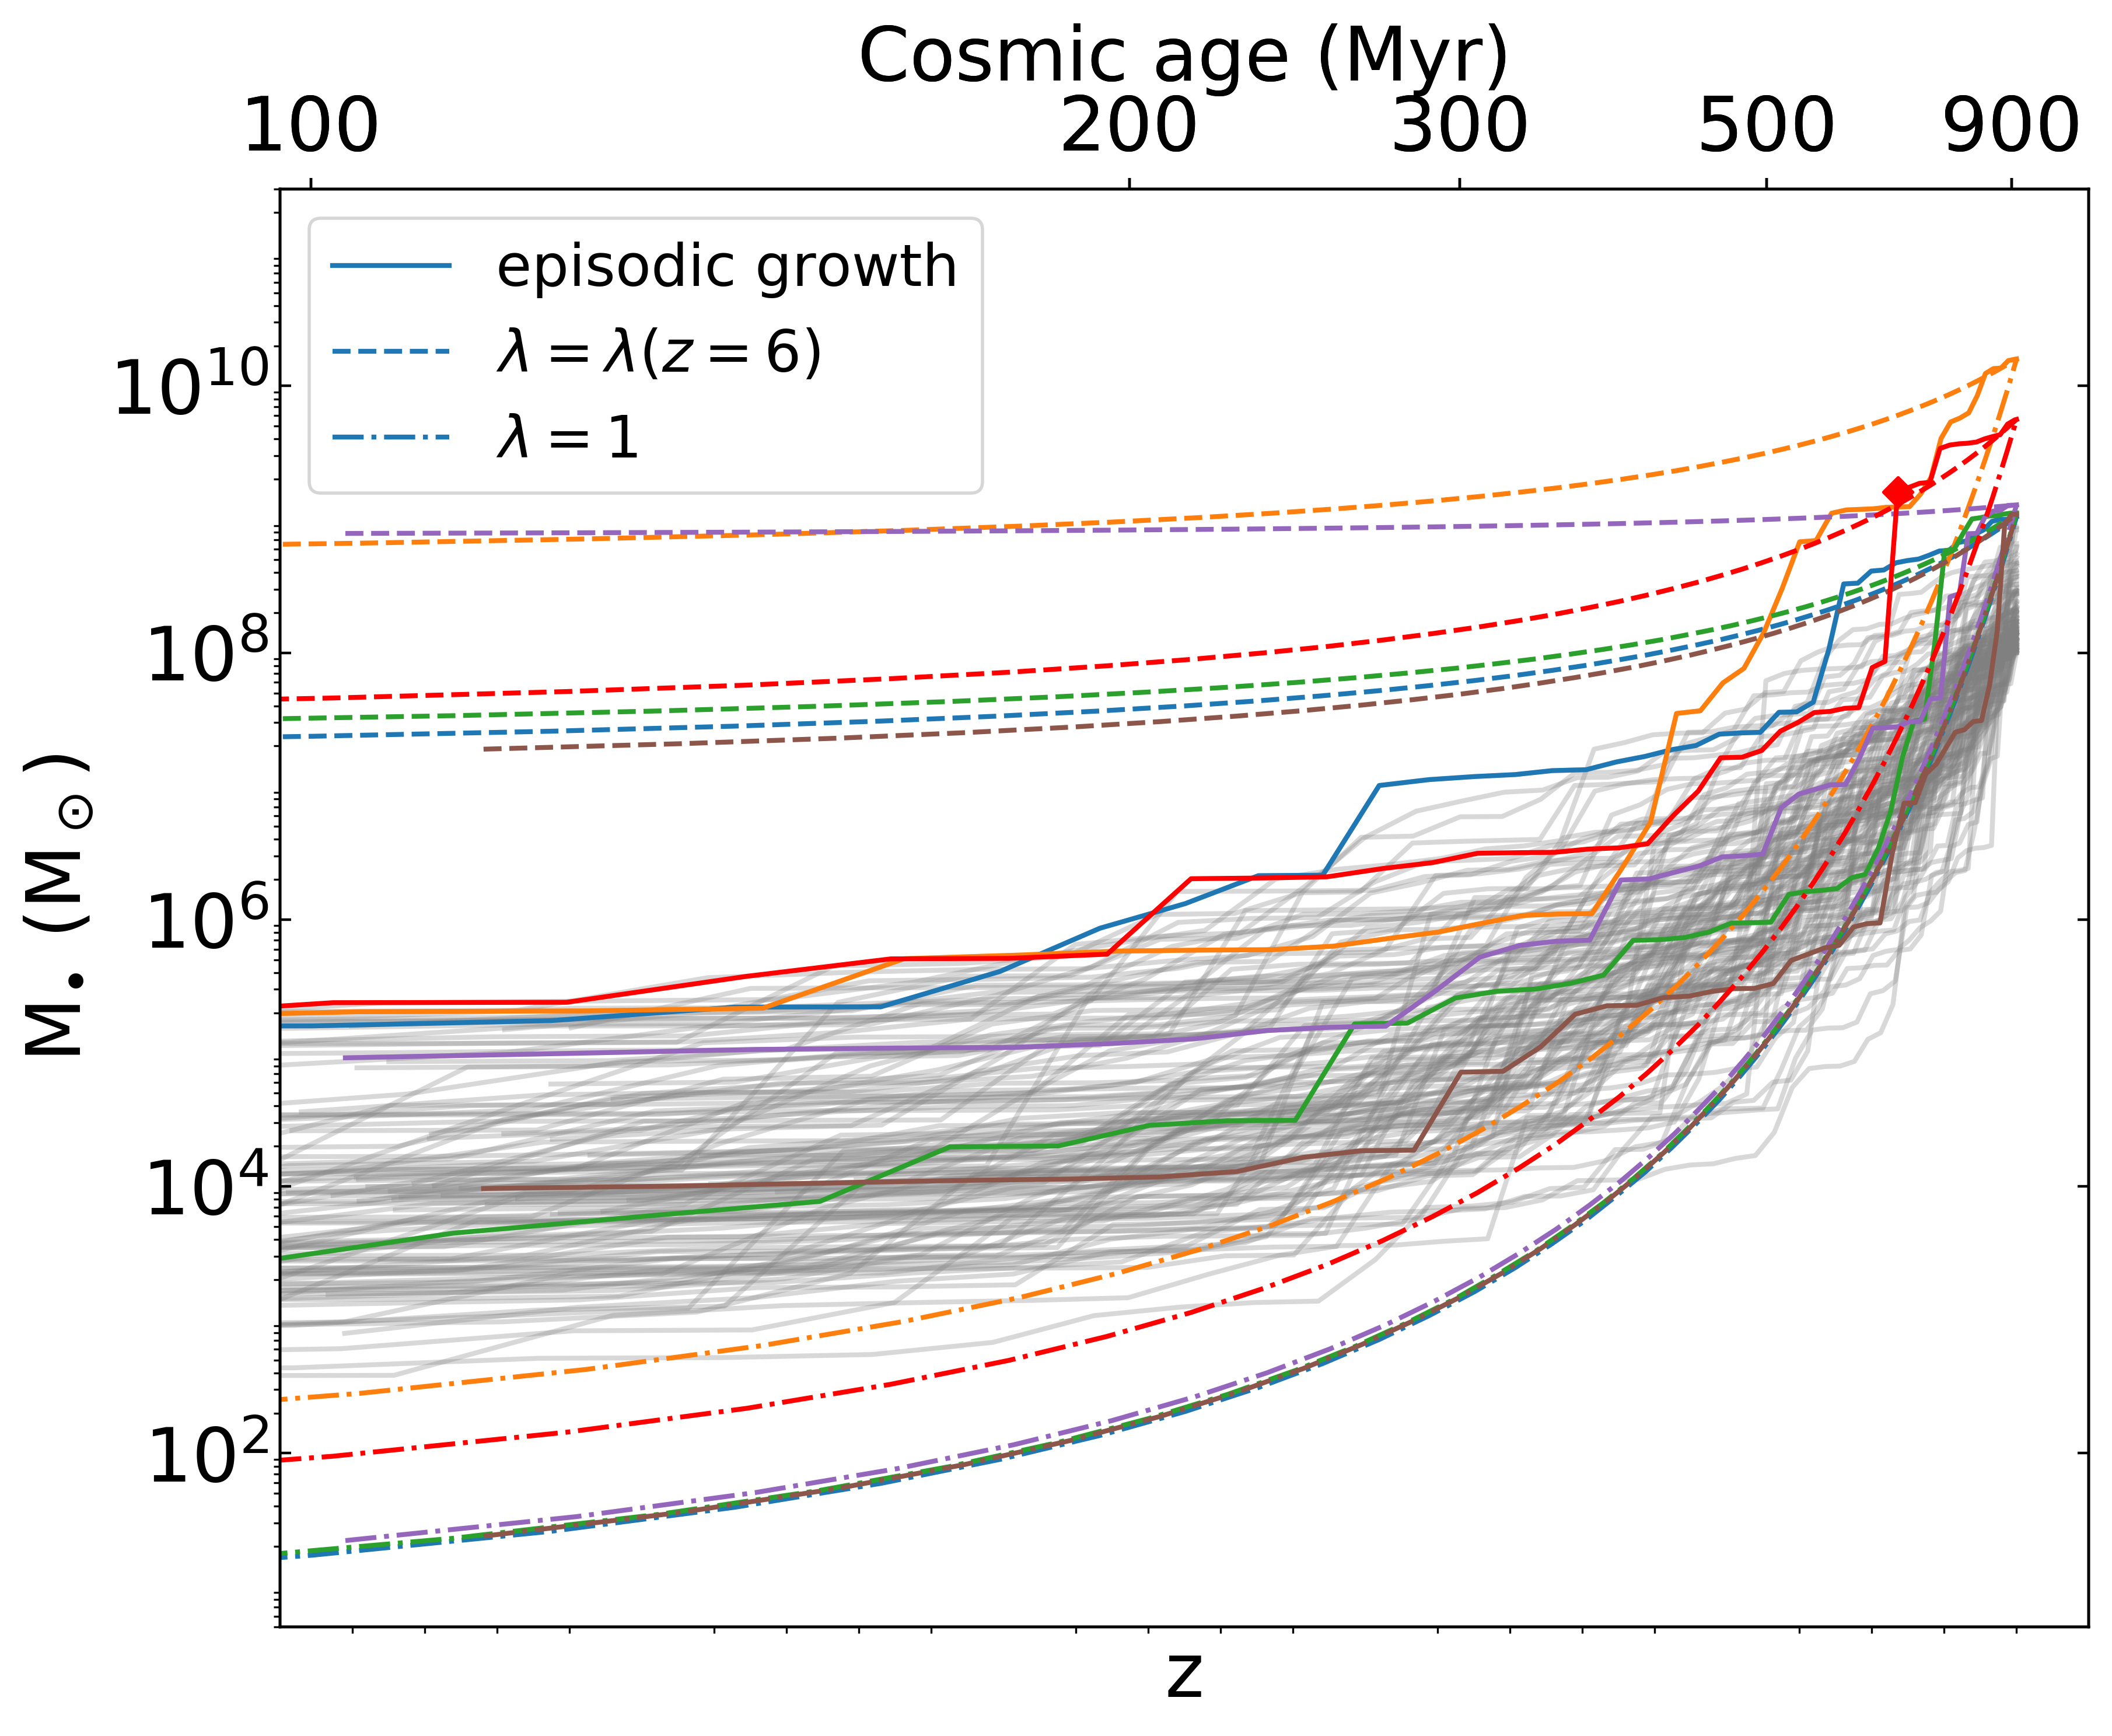
\includegraphics[width=85mm]{Mevol.png}
\caption{
Evolutionary tracks of individual seed BHs with the the best-fit growth model parameters in the $\fseed=0.01$ case.
Among all the samples, we select BHs that reach $M\geq 10^8~\Msun$ at $z=6$ (solid curves). 
The heaviest 7 BHs with $M_\bullet \geq 10^9~\Msun$ at $z=6$ are highlighted with colors. 
For the heaviest BHs, we draw the assembly history assuming an exponential growth with a constant Eddington ratio: 
the $\lambda$-value found at $z=6$ for each BH (dotted curves; extrapolation with an observed value of $\lambda$) and 
$\lambda =1$ (dashed curves; continuous Eddington growth).
%constant $\lambda$ keeping the $z=$ 6 value with dotted lines and 
%Eddington limit growth with $\lambda=1$ with dashed lines.
}
\label{fig:track}
\end{figure}



\vspace{2mm}
\subsection{The distribution of the Eddington ratio: \\observed v.s. underlying populations}\label{sec:ldist}

It is challenging to discuss the properties of the underlying quasar population
%Discussion on quasar \textit{intrinsic} properties is naturally difficult, 
because observed quasars are selected based on some criteria, e.g., the limiting magnitude.
%a cut off of detection under some magnitude floor. 
The unavoidable bias of quasar surveys could be corrected with the selection function calibrated
by experiments on the detectability of mock data, but is not fully solved. 
In this section, we examine the effect of flux-limited quasar surveys on the observed ERDF, 
taking advantage of our complete sample of high-$z$ BH populations in the whole luminosity range. 


Based on the quasar sample from the best-fit model described in \S~\ref{sec:evol}, 
we select quasars with a bolometric luminosity cut.
%of $\Lbol \geq 10^{46}~\mathrm{erg~s^{-1}}$. 
In Fig.~\ref{fig:lhist}, we present the intrinsic ERDFs for the whole BH sample (blue) and the selected sample with
a luminosity cut of $\Lbol \geq 10^{46}~\mathrm{erg~s^{-1}}$ (green) and $\Lbol \geq 10^{45}~\mathrm{erg~s^{-1}}$ (orange).  
The Eddington ratio for the whole sample follows a Schechter shape with a majority of inactive quasars, 
while the observed Eddington ratio is biased toward higher values and the distribution results in a log-normal shape. 
The latter distribution is presented by various observational efforts in the $z\sim$ 6 brightest quasar samples 
\citep[e.g.,][]{2010AJ....140..546W,2019ApJ...873...35S}.
However, our best-fit growth model reproducing both the BHMF and QLF at $z\sim$ 6 suggests the existence of
a large number of underlying BH populations with low Eddington ratios. 
%based on the best-fit growth model connecting the BH seeding and $z\sim$ 6 BHMF and QLF. 
We find that the log-normal shape still holds with the lower luminosity cut, 
%To demonstrate qualitatively the caveat for the detection limit on recovering the intrinsic quasar properties, 
%we also examine the observed ERDF by selecting quasars with $\Lbol>10^{45}~\mathrm{erg~s^{-1}}$. 
but a lower detection limit unveils more hidden quasars with low Eddington ratios. 
This will be proved by the ongoing observations with the Subaru HSC providing low-luminosity and less-massive BH samples
(Onoue et al. in prep).
%Therefore, we emphasize that it is imperative to lower the detection limit in order to 
%understand a more complete quasar sample at high-$z$, 
%so that the numerous dimly accreting BHs can be shed light on.



%%%%%%%
%    Fig. 7
%%%%%%%
\begin{figure}
\centering
\includegraphics[width=80mm]{distf2N5_06231122_l_hist.png}
\caption{
The intrinsic Eddington ratio distribution function for the whole BH sample (blue) and the selected sample with
a luminosity cut of $\Lbol \geq 10^{46}~\mathrm{erg~s^{-1}}$ (green) and $\Lbol \geq 10^{45}~\mathrm{erg~s^{-1}}$ (orange).  
%Intrinsic ERDF (blue) and the observed ones after imposing selection effects by $\Lbol>L_\mathrm{lim}=10^{45}$ (orange) and 10$^{46}$ erg~s$^{-1}$ (green).
The observed histograms are elevated by arbitrary normalizations for comparison of the distribution shapes.
The intrinsic ERDF follows the best-fitted Schechter function (dashed curve), 
while the observed ERDF with a detection limit imposed results in a log-normal shape, 
with a large low Eddington ratio quasars hidden from detection.
The log-normal shape still holds with the lower luminosity cut, 
but a lower detection limit alleviates the selection effect against the low Eddington ratio quasar populations.
%With decreasing $L_\mathrm{lim}$, more low $\lambda$ population is unveiled.
}
\label{fig:lhist}
\end{figure}
  


% \begin{acknowledgments}
% % We thank all the people that have made this paper what it is today.  
% % This includes but not limited to Bob Hanisch, Chris Biemesderfer, Lee Brotzman,
% % Pierre Landau, Arthur Ogawa, Maxim Markevitch, Alexey Vikhlinin and Amy
% % Hendrickson. Also special thanks to David Hogg and Daniel Foreman-Mackey
% % for the new "modern" style design. Considerable help was provided via bug
% % reports and hacks from numerous people including Patriciddo Cubillos, Alex
% % Drlica-Wagner, Sean Lake, Michele Bannister, Peter Williams, and Jonathan
% % Gagne.
% \end{acknowledgments}

%% To help institutions obtain information on the effectiveness of their 
%% telescopes the AAS Journals has created a group of keywords for telescope 
%% facilities.
%
%% Following the acknowledgments section, use the following syntax and the
%% \facility{} or \facilities{} macros to list the keywords of facilities used 
%% in the research for the paper.  Each keyword is check against the master 
%% list during copy editing.  Individual instruments can be provided in 
%% parentheses, after the keyword, but they are not verified.


% \facilities{HST(STIS), Swift(XRT and UVOT), AAVSO, CTIO:1.3m, CTIO:1.5m,CXO}

%% Similar to \facility{}, there is the optional \software command to allow 
%% authors a place to specify which programs were used during the creation of 
%% the manuscript. Authors should list each code and include either a
%% citation or url to the code inside ()s when available.

% \software{astropy \citep{2013A&A...558A..33A,2018AJ....156..123A},  
%           Cloudy \citep{2013RMxAA..49..137F}, 
%           Source Extractor \citep{1996A&AS..117..393B}
%           }

%% Appendix material should be preceded with a single \appendix command.
%% There should be a \section command for each appendix. Mark appendix
%% subsections with the same markup you use in the main body of the paper.

%% Each Appendix (indicated with \section) will be lettered A, B, C, etc.
%% The equation counter will reset when it encounters the \appendix
%% command and will number appendix equations (A1), (A2), etc. The
%% Figure and Table counter will not reset.

%% For this sample we use BibTeX plus aasjournals.bst to generate the
%% the bibliography. The sample631.bib file was populated from ADS. To
%% get the citations to show in the compiled file do the following:
%%
%% pdflatex sample631.tex
%% bibtext sample631
%% pdflatex sample631.tex
%% pdflatex sample631.tex

\clearpage

\newpage
% \vspace{100mm}
\bibliography{ref}{}
\bibliographystyle{aasjournal}

%% This command is needed to show the entire author+affiliation list when
%% the collaboration and author truncation commands are used.  It has to
%% go at the end of the manuscript.
%\allauthors

%% Include this line if you are using the \added, \replaced, \deleted
%% commands to see a summary list of all changes at the end of the article.
%\listofchanges

\end{CJK*}
\end{document}

% End of file `sample631.tex'.
